\documentclass{book}
\usepackage[a4paper,top=2.5cm,bottom=2.5cm,left=2.5cm,right=2.5cm]{geometry}
\usepackage{makeidx}
\usepackage{natbib}
\usepackage{graphicx}
\usepackage{multicol}
\usepackage{float}
\usepackage{listings}
\usepackage{color}
\usepackage{ifthen}
\usepackage[table]{xcolor}
\usepackage{textcomp}
\usepackage{alltt}
\usepackage{ifpdf}
\ifpdf
\usepackage[pdftex,
            pagebackref=true,
            colorlinks=true,
            linkcolor=blue,
            unicode
           ]{hyperref}
\else
\usepackage[ps2pdf,
            pagebackref=true,
            colorlinks=true,
            linkcolor=blue,
            unicode
           ]{hyperref}
\usepackage{pspicture}
\fi
\usepackage[utf8]{inputenc}
\usepackage{mathptmx}
\usepackage[scaled=.90]{helvet}
\usepackage{courier}
\usepackage{sectsty}
\usepackage{amssymb}
\usepackage[titles]{tocloft}
\usepackage{doxygen}
\lstset{language=C++,inputencoding=utf8,basicstyle=\footnotesize,breaklines=true,breakatwhitespace=true,tabsize=8,numbers=left }
\makeindex
\setcounter{tocdepth}{3}
\renewcommand{\footrulewidth}{0.4pt}
\renewcommand{\familydefault}{\sfdefault}
\hfuzz=15pt
\setlength{\emergencystretch}{15pt}
\hbadness=750
\tolerance=750
\begin{document}
\hypersetup{pageanchor=false,citecolor=blue}
\begin{titlepage}
\vspace*{7cm}
\begin{center}
{\Large My Project }\\
\vspace*{1cm}
{\large Generated by Doxygen 1.8.1.2}\\
\vspace*{0.5cm}
{\small Tue Dec 17 2013 18:33:04}\\
\end{center}
\end{titlepage}
\clearemptydoublepage
\pagenumbering{roman}
\tableofcontents
\clearemptydoublepage
\pagenumbering{arabic}
\hypersetup{pageanchor=true,citecolor=blue}
\chapter{R\-E\-A\-D\-M\-E}
\label{md_README}
\hypertarget{md_README}{}
\input{md_README}
\chapter{Class Index}
\section{Class Hierarchy}
This inheritance list is sorted roughly, but not completely, alphabetically\-:\begin{DoxyCompactList}
\item \contentsline{section}{Ace\-Val}{\pageref{classAceVal}}{}
\item \contentsline{section}{D\-B\-Connection}{\pageref{classDBConnection}}{}
\item \contentsline{section}{D\-Bthread}{\pageref{classDBthread}}{}
\item \contentsline{section}{Frame}{\pageref{structFrame}}{}
\item \contentsline{section}{New\-D\-B}{\pageref{classNewDB}}{}
\item \contentsline{section}{pipeline}{\pageref{classpipeline}}{}
\item \contentsline{section}{Player}{\pageref{classPlayer}}{}
\item \contentsline{section}{Player\-Dialog}{\pageref{classPlayerDialog}}{}
\item \contentsline{section}{Players\-Control}{\pageref{classPlayersControl}}{}
\item \contentsline{section}{Scene}{\pageref{classScene}}{}
\item \contentsline{section}{Scene\-Dialog}{\pageref{classSceneDialog}}{}
\item \contentsline{section}{Ui\-\_\-\-Ace\-Val}{\pageref{classUi__AceVal}}{}
\begin{DoxyCompactList}
\item \contentsline{section}{Ui\-:\-:Ace\-Val}{\pageref{classUi_1_1AceVal}}{}
\end{DoxyCompactList}
\item \contentsline{section}{Ui\-\_\-\-D\-B\-Connection}{\pageref{classUi__DBConnection}}{}
\begin{DoxyCompactList}
\item \contentsline{section}{Ui\-:\-:D\-B\-Connection}{\pageref{classUi_1_1DBConnection}}{}
\end{DoxyCompactList}
\item \contentsline{section}{Ui\-\_\-\-Dialog}{\pageref{classUi__Dialog}}{}
\begin{DoxyCompactList}
\item \contentsline{section}{Ui\-:\-:Dialog}{\pageref{classUi_1_1Dialog}}{}
\end{DoxyCompactList}
\item \contentsline{section}{Ui\-\_\-\-New\-D\-B}{\pageref{classUi__NewDB}}{}
\begin{DoxyCompactList}
\item \contentsline{section}{Ui\-:\-:New\-D\-B}{\pageref{classUi_1_1NewDB}}{}
\end{DoxyCompactList}
\item \contentsline{section}{Ui\-\_\-\-Player\-Dialog}{\pageref{classUi__PlayerDialog}}{}
\begin{DoxyCompactList}
\item \contentsline{section}{Ui\-:\-:Player\-Dialog}{\pageref{classUi_1_1PlayerDialog}}{}
\end{DoxyCompactList}
\item \contentsline{section}{Ui\-\_\-\-Players\-Control}{\pageref{classUi__PlayersControl}}{}
\begin{DoxyCompactList}
\item \contentsline{section}{Ui\-:\-:Players\-Control}{\pageref{classUi_1_1PlayersControl}}{}
\end{DoxyCompactList}
\item \contentsline{section}{Ui\-\_\-\-Scene\-Dialog}{\pageref{classUi__SceneDialog}}{}
\begin{DoxyCompactList}
\item \contentsline{section}{Ui\-:\-:Scene\-Dialog}{\pageref{classUi_1_1SceneDialog}}{}
\end{DoxyCompactList}
\end{DoxyCompactList}

\chapter{Class Index}
\section{Class List}
Here are the classes, structs, unions and interfaces with brief descriptions\-:\begin{DoxyCompactList}
\item\contentsline{section}{\hyperlink{classAceVal}{Ace\-Val} }{\pageref{classAceVal}}{}
\item\contentsline{section}{\hyperlink{classUi_1_1AceVal}{Ui\-::\-Ace\-Val} }{\pageref{classUi_1_1AceVal}}{}
\item\contentsline{section}{\hyperlink{classDBConnection}{D\-B\-Connection} }{\pageref{classDBConnection}}{}
\item\contentsline{section}{\hyperlink{classUi_1_1DBConnection}{Ui\-::\-D\-B\-Connection} }{\pageref{classUi_1_1DBConnection}}{}
\item\contentsline{section}{\hyperlink{classDBthread}{D\-Bthread} }{\pageref{classDBthread}}{}
\item\contentsline{section}{\hyperlink{classUi_1_1Dialog}{Ui\-::\-Dialog} }{\pageref{classUi_1_1Dialog}}{}
\item\contentsline{section}{\hyperlink{structFrame}{Frame} }{\pageref{structFrame}}{}
\item\contentsline{section}{\hyperlink{classUi_1_1NewDB}{Ui\-::\-New\-D\-B} }{\pageref{classUi_1_1NewDB}}{}
\item\contentsline{section}{\hyperlink{classNewDB}{New\-D\-B} }{\pageref{classNewDB}}{}
\item\contentsline{section}{\hyperlink{classpipeline}{pipeline} }{\pageref{classpipeline}}{}
\item\contentsline{section}{\hyperlink{classPlayer}{Player} }{\pageref{classPlayer}}{}
\item\contentsline{section}{\hyperlink{classPlayerDialog}{Player\-Dialog} }{\pageref{classPlayerDialog}}{}
\item\contentsline{section}{\hyperlink{classUi_1_1PlayerDialog}{Ui\-::\-Player\-Dialog} }{\pageref{classUi_1_1PlayerDialog}}{}
\item\contentsline{section}{\hyperlink{classPlayersControl}{Players\-Control} }{\pageref{classPlayersControl}}{}
\item\contentsline{section}{\hyperlink{classUi_1_1PlayersControl}{Ui\-::\-Players\-Control} }{\pageref{classUi_1_1PlayersControl}}{}
\item\contentsline{section}{\hyperlink{classScene}{Scene} }{\pageref{classScene}}{}
\item\contentsline{section}{\hyperlink{classSceneDialog}{Scene\-Dialog} }{\pageref{classSceneDialog}}{}
\item\contentsline{section}{\hyperlink{classUi_1_1SceneDialog}{Ui\-::\-Scene\-Dialog} }{\pageref{classUi_1_1SceneDialog}}{}
\item\contentsline{section}{\hyperlink{classUi__AceVal}{Ui\-\_\-\-Ace\-Val} }{\pageref{classUi__AceVal}}{}
\item\contentsline{section}{\hyperlink{classUi__DBConnection}{Ui\-\_\-\-D\-B\-Connection} }{\pageref{classUi__DBConnection}}{}
\item\contentsline{section}{\hyperlink{classUi__Dialog}{Ui\-\_\-\-Dialog} }{\pageref{classUi__Dialog}}{}
\item\contentsline{section}{\hyperlink{classUi__NewDB}{Ui\-\_\-\-New\-D\-B} }{\pageref{classUi__NewDB}}{}
\item\contentsline{section}{\hyperlink{classUi__PlayerDialog}{Ui\-\_\-\-Player\-Dialog} }{\pageref{classUi__PlayerDialog}}{}
\item\contentsline{section}{\hyperlink{classUi__PlayersControl}{Ui\-\_\-\-Players\-Control} }{\pageref{classUi__PlayersControl}}{}
\item\contentsline{section}{\hyperlink{classUi__SceneDialog}{Ui\-\_\-\-Scene\-Dialog} }{\pageref{classUi__SceneDialog}}{}
\end{DoxyCompactList}

\chapter{Class Documentation}
\hypertarget{classAceVal}{\section{Ace\-Val Class Reference}
\label{classAceVal}\index{Ace\-Val@{Ace\-Val}}
}
\subsection*{Signals}
\begin{DoxyCompactItemize}
\item 
\hypertarget{classAceVal_aecbf3b36ad3558dee489643c4c04af32}{void {\bfseries Connect} (Q\-String Host, Q\-String User, Q\-String Password)}\label{classAceVal_aecbf3b36ad3558dee489643c4c04af32}

\item 
\hypertarget{classAceVal_a5e1c5c9897361ce65c4b9bd2859035b5}{void {\bfseries open\-Thread\-D\-B} (Q\-String query)}\label{classAceVal_a5e1c5c9897361ce65c4b9bd2859035b5}

\item 
\hypertarget{classAceVal_ae7b32eeee7aa51c3630c9747d328eaf6}{void {\bfseries new\-D\-B\-Create} (Q\-String query, Q\-String D\-Bname)}\label{classAceVal_ae7b32eeee7aa51c3630c9747d328eaf6}

\item 
\hypertarget{classAceVal_a83b9e57722b3dac8a18f797792163a9a}{void {\bfseries store\-Info} (Q\-Vector$<$ \hyperlink{structFrame}{Frame} $>$ $\ast$frames\-To\-Insert)}\label{classAceVal_a83b9e57722b3dac8a18f797792163a9a}

\item 
\hypertarget{classAceVal_a42959e954aa90edebe5e25cf9cb2f907}{void {\bfseries store\-Players} (int start, int end, Q\-Vector$<$ \hyperlink{classPlayer}{Player} $>$ $\ast$players)}\label{classAceVal_a42959e954aa90edebe5e25cf9cb2f907}

\end{DoxyCompactItemize}
\subsection*{Public Member Functions}
\begin{DoxyCompactItemize}
\item 
\hyperlink{classAceVal_aa8c4668b26df05d2f237097b6161f903}{Ace\-Val} (Q\-Widget $\ast$parent=0)
\begin{DoxyCompactList}\small\item\em \hyperlink{classAceVal_aa8c4668b26df05d2f237097b6161f903}{Ace\-Val\-::\-Ace\-Val}. \end{DoxyCompactList}\item 
\hyperlink{classAceVal_a69f8950b854fc3579ebc1395054ba6dc}{$\sim$\-Ace\-Val} ()
\begin{DoxyCompactList}\small\item\em \hyperlink{classAceVal_a69f8950b854fc3579ebc1395054ba6dc}{Ace\-Val\-::$\sim$\-Ace\-Val}. \end{DoxyCompactList}\end{DoxyCompactItemize}
\subsection*{Public Attributes}
\begin{DoxyCompactItemize}
\item 
\hypertarget{classAceVal_ab10a71bf1f9196d258b72205a388ee8e}{\hyperlink{classpipeline}{pipeline} $\ast$ {\bfseries Pipeline}}\label{classAceVal_ab10a71bf1f9196d258b72205a388ee8e}

\item 
\hypertarget{classAceVal_a7b7d746e43c9607dfbfeaba07cc4e705}{Q\-Vector$<$ \hyperlink{classScene}{Scene} $>$ {\bfseries Scenes}}\label{classAceVal_a7b7d746e43c9607dfbfeaba07cc4e705}

\item 
\hypertarget{classAceVal_a5d30355e02ce19edd4d2dbddf5010f63}{Q\-Vector$<$ \hyperlink{classPlayer}{Player} $>$ {\bfseries Players}}\label{classAceVal_a5d30355e02ce19edd4d2dbddf5010f63}

\end{DoxyCompactItemize}


\subsection{Constructor \& Destructor Documentation}
\hypertarget{classAceVal_aa8c4668b26df05d2f237097b6161f903}{\index{Ace\-Val@{Ace\-Val}!Ace\-Val@{Ace\-Val}}
\index{Ace\-Val@{Ace\-Val}!AceVal@{Ace\-Val}}
\subsubsection[{Ace\-Val}]{\setlength{\rightskip}{0pt plus 5cm}Ace\-Val\-::\-Ace\-Val (
\begin{DoxyParamCaption}
\item[{Q\-Widget $\ast$}]{parent = {\ttfamily 0}}
\end{DoxyParamCaption}
)\hspace{0.3cm}{\ttfamily [explicit]}}}\label{classAceVal_aa8c4668b26df05d2f237097b6161f903}


\hyperlink{classAceVal_aa8c4668b26df05d2f237097b6161f903}{Ace\-Val\-::\-Ace\-Val}. 


\begin{DoxyParams}{Parameters}
{\em parent} & This class is the main implementation of the application, it contains all the controls for the tracking, also it stablishes the connection with the sql database in order to store the results \\
\hline
\end{DoxyParams}
\hypertarget{classAceVal_a69f8950b854fc3579ebc1395054ba6dc}{\index{Ace\-Val@{Ace\-Val}!$\sim$\-Ace\-Val@{$\sim$\-Ace\-Val}}
\index{$\sim$\-Ace\-Val@{$\sim$\-Ace\-Val}!AceVal@{Ace\-Val}}
\subsubsection[{$\sim$\-Ace\-Val}]{\setlength{\rightskip}{0pt plus 5cm}Ace\-Val\-::$\sim$\-Ace\-Val (
\begin{DoxyParamCaption}
{}
\end{DoxyParamCaption}
)}}\label{classAceVal_a69f8950b854fc3579ebc1395054ba6dc}


\hyperlink{classAceVal_a69f8950b854fc3579ebc1395054ba6dc}{Ace\-Val\-::$\sim$\-Ace\-Val}. 

Destructor created by qt 

The documentation for this class was generated from the following files\-:\begin{DoxyCompactItemize}
\item 
aceval.\-h\item 
aceval.\-cpp\item 
moc\-\_\-aceval.\-cpp\end{DoxyCompactItemize}

\hypertarget{classUi_1_1AceVal}{\section{Ui\-:\-:Ace\-Val Class Reference}
\label{classUi_1_1AceVal}\index{Ui\-::\-Ace\-Val@{Ui\-::\-Ace\-Val}}
}
Inheritance diagram for Ui\-:\-:Ace\-Val\-:\begin{figure}[H]
\begin{center}
\leavevmode
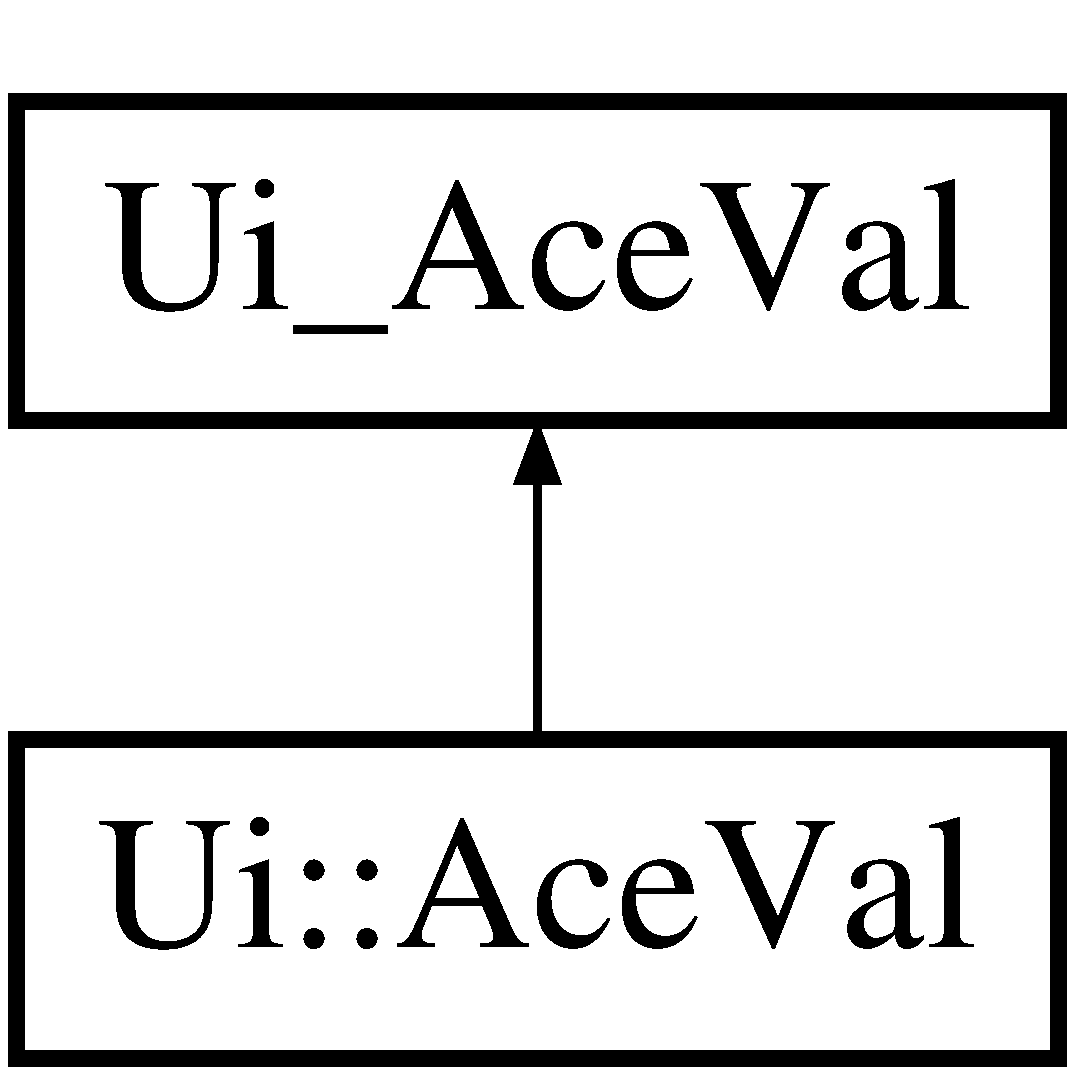
\includegraphics[height=2.000000cm]{classUi_1_1AceVal}
\end{center}
\end{figure}
\subsection*{Additional Inherited Members}


The documentation for this class was generated from the following file\-:\begin{DoxyCompactItemize}
\item 
ui\-\_\-aceval.\-h\end{DoxyCompactItemize}

\hypertarget{classDBConnection}{\section{D\-B\-Connection Class Reference}
\label{classDBConnection}\index{D\-B\-Connection@{D\-B\-Connection}}
}
\subsection*{Public Member Functions}
\begin{DoxyCompactItemize}
\item 
\hyperlink{classDBConnection_a1b38e96a988c6d7f530bb3aa6a8fc3a8}{D\-B\-Connection} (Q\-Widget $\ast$parent=0)
\begin{DoxyCompactList}\small\item\em \hyperlink{classDBConnection_a1b38e96a988c6d7f530bb3aa6a8fc3a8}{D\-B\-Connection\-::\-D\-B\-Connection}. \end{DoxyCompactList}\item 
\hypertarget{classDBConnection_ae21031a13c223440f5af5c62dc4bc84c}{\hyperlink{classDBConnection_ae21031a13c223440f5af5c62dc4bc84c}{$\sim$\-D\-B\-Connection} ()}\label{classDBConnection_ae21031a13c223440f5af5c62dc4bc84c}

\begin{DoxyCompactList}\small\item\em \hyperlink{classDBConnection_ae21031a13c223440f5af5c62dc4bc84c}{D\-B\-Connection\-::$\sim$\-D\-B\-Connection} \hyperlink{classDBConnection}{D\-B\-Connection} destructor created by qt. \end{DoxyCompactList}\item 
Q\-String \hyperlink{classDBConnection_a6477ddffd0a1439ecf0dfed6ebf17c14}{get\-Host\-Name} ()
\begin{DoxyCompactList}\small\item\em \hyperlink{classDBConnection_a6477ddffd0a1439ecf0dfed6ebf17c14}{D\-B\-Connection\-::get\-Host\-Name}. \end{DoxyCompactList}\item 
Q\-String \hyperlink{classDBConnection_a9b68b9e34a5602f621f2208977f35d68}{get\-User} ()
\begin{DoxyCompactList}\small\item\em \hyperlink{classDBConnection_a9b68b9e34a5602f621f2208977f35d68}{D\-B\-Connection\-::get\-User}. \end{DoxyCompactList}\item 
Q\-String \hyperlink{classDBConnection_a44b98126e3511f201585a619f3dc2204}{get\-Password} ()
\begin{DoxyCompactList}\small\item\em \hyperlink{classDBConnection_a44b98126e3511f201585a619f3dc2204}{D\-B\-Connection\-::get\-Password}. \end{DoxyCompactList}\end{DoxyCompactItemize}


\subsection{Constructor \& Destructor Documentation}
\hypertarget{classDBConnection_a1b38e96a988c6d7f530bb3aa6a8fc3a8}{\index{D\-B\-Connection@{D\-B\-Connection}!D\-B\-Connection@{D\-B\-Connection}}
\index{D\-B\-Connection@{D\-B\-Connection}!DBConnection@{D\-B\-Connection}}
\subsubsection[{D\-B\-Connection}]{\setlength{\rightskip}{0pt plus 5cm}D\-B\-Connection\-::\-D\-B\-Connection (
\begin{DoxyParamCaption}
\item[{Q\-Widget $\ast$}]{parent = {\ttfamily 0}}
\end{DoxyParamCaption}
)\hspace{0.3cm}{\ttfamily [explicit]}}}\label{classDBConnection_a1b38e96a988c6d7f530bb3aa6a8fc3a8}


\hyperlink{classDBConnection_a1b38e96a988c6d7f530bb3aa6a8fc3a8}{D\-B\-Connection\-::\-D\-B\-Connection}. 


\begin{DoxyParams}{Parameters}
{\em parent} & Building the connection dialog for creating a link with D\-B driver. \\
\hline
\end{DoxyParams}


\subsection{Member Function Documentation}
\hypertarget{classDBConnection_a6477ddffd0a1439ecf0dfed6ebf17c14}{\index{D\-B\-Connection@{D\-B\-Connection}!get\-Host\-Name@{get\-Host\-Name}}
\index{get\-Host\-Name@{get\-Host\-Name}!DBConnection@{D\-B\-Connection}}
\subsubsection[{get\-Host\-Name}]{\setlength{\rightskip}{0pt plus 5cm}Q\-String D\-B\-Connection\-::get\-Host\-Name (
\begin{DoxyParamCaption}
{}
\end{DoxyParamCaption}
)}}\label{classDBConnection_a6477ddffd0a1439ecf0dfed6ebf17c14}


\hyperlink{classDBConnection_a6477ddffd0a1439ecf0dfed6ebf17c14}{D\-B\-Connection\-::get\-Host\-Name}. 

\begin{DoxyReturn}{Returns}
the host name Public function for accesing the hostname attribute 
\end{DoxyReturn}
\hypertarget{classDBConnection_a44b98126e3511f201585a619f3dc2204}{\index{D\-B\-Connection@{D\-B\-Connection}!get\-Password@{get\-Password}}
\index{get\-Password@{get\-Password}!DBConnection@{D\-B\-Connection}}
\subsubsection[{get\-Password}]{\setlength{\rightskip}{0pt plus 5cm}Q\-String D\-B\-Connection\-::get\-Password (
\begin{DoxyParamCaption}
{}
\end{DoxyParamCaption}
)}}\label{classDBConnection_a44b98126e3511f201585a619f3dc2204}


\hyperlink{classDBConnection_a44b98126e3511f201585a619f3dc2204}{D\-B\-Connection\-::get\-Password}. 

\begin{DoxyReturn}{Returns}
The db password Public function for accesing the password attribute. 
\end{DoxyReturn}
\hypertarget{classDBConnection_a9b68b9e34a5602f621f2208977f35d68}{\index{D\-B\-Connection@{D\-B\-Connection}!get\-User@{get\-User}}
\index{get\-User@{get\-User}!DBConnection@{D\-B\-Connection}}
\subsubsection[{get\-User}]{\setlength{\rightskip}{0pt plus 5cm}Q\-String D\-B\-Connection\-::get\-User (
\begin{DoxyParamCaption}
{}
\end{DoxyParamCaption}
)}}\label{classDBConnection_a9b68b9e34a5602f621f2208977f35d68}


\hyperlink{classDBConnection_a9b68b9e34a5602f621f2208977f35d68}{D\-B\-Connection\-::get\-User}. 

\begin{DoxyReturn}{Returns}
The user name Public function for accesing the username attribute 
\end{DoxyReturn}


The documentation for this class was generated from the following files\-:\begin{DoxyCompactItemize}
\item 
dbconnection.\-h\item 
dbconnection.\-cpp\end{DoxyCompactItemize}

\hypertarget{classUi_1_1DBConnection}{\section{Ui\-:\-:D\-B\-Connection Class Reference}
\label{classUi_1_1DBConnection}\index{Ui\-::\-D\-B\-Connection@{Ui\-::\-D\-B\-Connection}}
}
Inheritance diagram for Ui\-:\-:D\-B\-Connection\-:\begin{figure}[H]
\begin{center}
\leavevmode
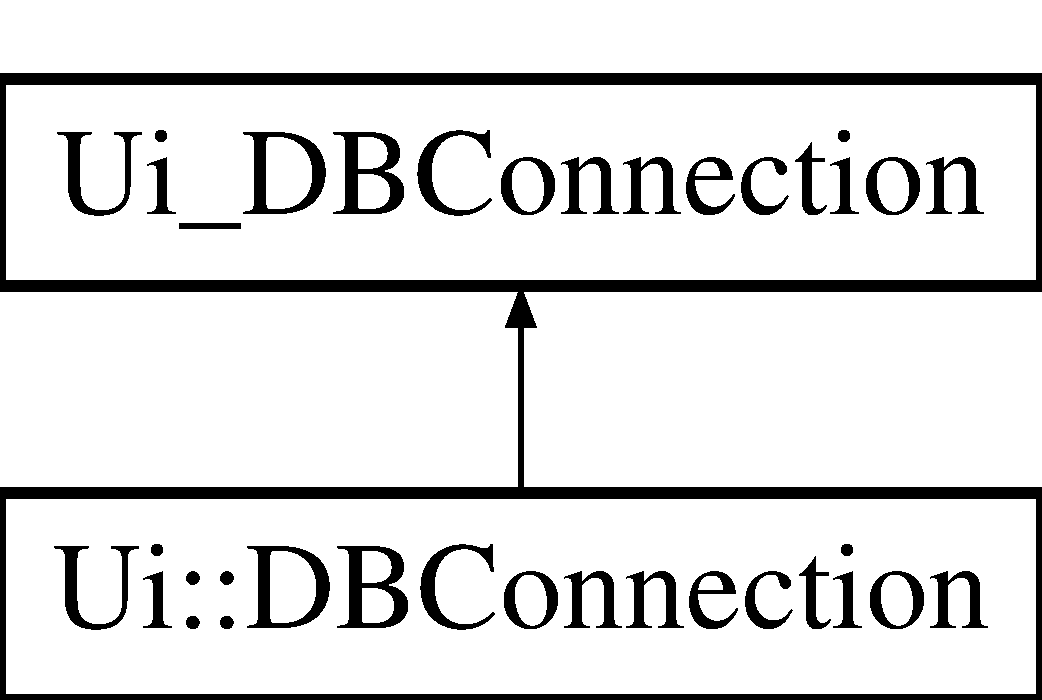
\includegraphics[height=2.000000cm]{classUi_1_1DBConnection}
\end{center}
\end{figure}
\subsection*{Additional Inherited Members}


The documentation for this class was generated from the following file\-:\begin{DoxyCompactItemize}
\item 
ui\-\_\-dbconnection.\-h\end{DoxyCompactItemize}

\hypertarget{classDBthread}{\section{D\-Bthread Class Reference}
\label{classDBthread}\index{D\-Bthread@{D\-Bthread}}
}
\subsection*{Public Slots}
\begin{DoxyCompactItemize}
\item 
void \hyperlink{classDBthread_a2dbcf7890c95b1fca26f9bd21d054e46}{connect\-D\-B} (Q\-String Host, Q\-String User, Q\-String Password)
\begin{DoxyCompactList}\small\item\em \hyperlink{classDBthread_a2dbcf7890c95b1fca26f9bd21d054e46}{D\-Bthread\-::connect\-D\-B}. \end{DoxyCompactList}\item 
void \hyperlink{classDBthread_a355e688d4a6f590578f2c29f468b3ad0}{open\-D\-B} (Q\-String query)
\begin{DoxyCompactList}\small\item\em \hyperlink{classDBthread_a355e688d4a6f590578f2c29f468b3ad0}{D\-Bthread\-::open\-D\-B}. \end{DoxyCompactList}\item 
void \hyperlink{classDBthread_a86757b487ce90e3589334d6f96dc6684}{new\-D\-B} (Q\-String query, Q\-String D\-Bname)
\begin{DoxyCompactList}\small\item\em \hyperlink{classDBthread_a86757b487ce90e3589334d6f96dc6684}{D\-Bthread\-::new\-D\-B}. \end{DoxyCompactList}\item 
void \hyperlink{classDBthread_ad5e320be8718aa773eeab3303ceb9d07}{store\-Infor} (Q\-Vector$<$ \hyperlink{structFrame}{Frame} $>$ $\ast$frames\-To\-Insert)
\begin{DoxyCompactList}\small\item\em \hyperlink{classDBthread_ad5e320be8718aa773eeab3303ceb9d07}{D\-Bthread\-::store\-Infor}. \end{DoxyCompactList}\item 
void \hyperlink{classDBthread_a37468e05639656f8a6d9f69a3937676e}{store\-Players} (int start, int end, Q\-Vector$<$ \hyperlink{classPlayer}{Player} $>$ $\ast$players)
\begin{DoxyCompactList}\small\item\em \hyperlink{classDBthread_a37468e05639656f8a6d9f69a3937676e}{D\-Bthread\-::store\-Players}. \end{DoxyCompactList}\end{DoxyCompactItemize}
\subsection*{Signals}
\begin{DoxyCompactItemize}
\item 
\hypertarget{classDBthread_a7b9df87143f9f5d108a8b7ac59c83af0}{void {\bfseries connected} (bool is\-Connected)}\label{classDBthread_a7b9df87143f9f5d108a8b7ac59c83af0}

\item 
\hypertarget{classDBthread_ab7de01fe14f319807df639a50160f107}{void {\bfseries open\-D\-B\-Fail} (bool result)}\label{classDBthread_ab7de01fe14f319807df639a50160f107}

\item 
\hypertarget{classDBthread_ac905b36e66201d6b8bb99de32525a251}{void {\bfseries quer\-Result} (bool result, Q\-String Error)}\label{classDBthread_ac905b36e66201d6b8bb99de32525a251}

\end{DoxyCompactItemize}
\subsection*{Public Member Functions}
\begin{DoxyCompactItemize}
\item 
\hyperlink{classDBthread_aaaf33aa07a311b3fb1711b30de85a0b4}{D\-Bthread} (Q\-Object $\ast$parent=0)
\begin{DoxyCompactList}\small\item\em \hyperlink{classDBthread_aaaf33aa07a311b3fb1711b30de85a0b4}{D\-Bthread\-::\-D\-Bthread}. \end{DoxyCompactList}\item 
\hyperlink{classDBthread_a7efeaae535038f72e32a52f3e69f987c}{$\sim$\-D\-Bthread} ()
\begin{DoxyCompactList}\small\item\em \hyperlink{classDBthread_a7efeaae535038f72e32a52f3e69f987c}{D\-Bthread\-::$\sim$\-D\-Bthread}. \end{DoxyCompactList}\item 
\hypertarget{classDBthread_a63cdd2ec0573009c2d28985a155e7a6a}{void {\bfseries run} ()}\label{classDBthread_a63cdd2ec0573009c2d28985a155e7a6a}

\end{DoxyCompactItemize}


\subsection{Constructor \& Destructor Documentation}
\hypertarget{classDBthread_aaaf33aa07a311b3fb1711b30de85a0b4}{\index{D\-Bthread@{D\-Bthread}!D\-Bthread@{D\-Bthread}}
\index{D\-Bthread@{D\-Bthread}!DBthread@{D\-Bthread}}
\subsubsection[{D\-Bthread}]{\setlength{\rightskip}{0pt plus 5cm}D\-Bthread\-::\-D\-Bthread (
\begin{DoxyParamCaption}
\item[{Q\-Object $\ast$}]{parent = {\ttfamily 0}}
\end{DoxyParamCaption}
)\hspace{0.3cm}{\ttfamily [explicit]}}}\label{classDBthread_aaaf33aa07a311b3fb1711b30de85a0b4}


\hyperlink{classDBthread_aaaf33aa07a311b3fb1711b30de85a0b4}{D\-Bthread\-::\-D\-Bthread}. 


\begin{DoxyParams}{Parameters}
{\em parent} & Constructor for building the \hyperlink{classDBthread}{D\-Bthread}, initializes the db driver. \\
\hline
\end{DoxyParams}
\hypertarget{classDBthread_a7efeaae535038f72e32a52f3e69f987c}{\index{D\-Bthread@{D\-Bthread}!$\sim$\-D\-Bthread@{$\sim$\-D\-Bthread}}
\index{$\sim$\-D\-Bthread@{$\sim$\-D\-Bthread}!DBthread@{D\-Bthread}}
\subsubsection[{$\sim$\-D\-Bthread}]{\setlength{\rightskip}{0pt plus 5cm}D\-Bthread\-::$\sim$\-D\-Bthread (
\begin{DoxyParamCaption}
{}
\end{DoxyParamCaption}
)}}\label{classDBthread_a7efeaae535038f72e32a52f3e69f987c}


\hyperlink{classDBthread_a7efeaae535038f72e32a52f3e69f987c}{D\-Bthread\-::$\sim$\-D\-Bthread}. 

Destructor for the \hyperlink{classDBthread}{D\-Bthread} removes the db driver. 

\subsection{Member Function Documentation}
\hypertarget{classDBthread_a2dbcf7890c95b1fca26f9bd21d054e46}{\index{D\-Bthread@{D\-Bthread}!connect\-D\-B@{connect\-D\-B}}
\index{connect\-D\-B@{connect\-D\-B}!DBthread@{D\-Bthread}}
\subsubsection[{connect\-D\-B}]{\setlength{\rightskip}{0pt plus 5cm}void D\-Bthread\-::connect\-D\-B (
\begin{DoxyParamCaption}
\item[{Q\-String}]{Host, }
\item[{Q\-String}]{User, }
\item[{Q\-String}]{Password}
\end{DoxyParamCaption}
)\hspace{0.3cm}{\ttfamily [slot]}}}\label{classDBthread_a2dbcf7890c95b1fca26f9bd21d054e46}


\hyperlink{classDBthread_a2dbcf7890c95b1fca26f9bd21d054e46}{D\-Bthread\-::connect\-D\-B}. 


\begin{DoxyParams}{Parameters}
{\em Host} & \\
\hline
{\em User} & \\
\hline
{\em Password} & Slot for communicating with the main thread and starting the database \\
\hline
\end{DoxyParams}
\hypertarget{classDBthread_a86757b487ce90e3589334d6f96dc6684}{\index{D\-Bthread@{D\-Bthread}!new\-D\-B@{new\-D\-B}}
\index{new\-D\-B@{new\-D\-B}!DBthread@{D\-Bthread}}
\subsubsection[{new\-D\-B}]{\setlength{\rightskip}{0pt plus 5cm}void D\-Bthread\-::new\-D\-B (
\begin{DoxyParamCaption}
\item[{Q\-String}]{query, }
\item[{Q\-String}]{D\-Bname}
\end{DoxyParamCaption}
)\hspace{0.3cm}{\ttfamily [slot]}}}\label{classDBthread_a86757b487ce90e3589334d6f96dc6684}


\hyperlink{classDBthread_a86757b487ce90e3589334d6f96dc6684}{D\-Bthread\-::new\-D\-B}. 


\begin{DoxyParams}{Parameters}
{\em query} & \\
\hline
{\em D\-Bname} & Slot for creating a new db and all the tables needed inside it. \\
\hline
\end{DoxyParams}
\hypertarget{classDBthread_a355e688d4a6f590578f2c29f468b3ad0}{\index{D\-Bthread@{D\-Bthread}!open\-D\-B@{open\-D\-B}}
\index{open\-D\-B@{open\-D\-B}!DBthread@{D\-Bthread}}
\subsubsection[{open\-D\-B}]{\setlength{\rightskip}{0pt plus 5cm}void D\-Bthread\-::open\-D\-B (
\begin{DoxyParamCaption}
\item[{Q\-String}]{query}
\end{DoxyParamCaption}
)\hspace{0.3cm}{\ttfamily [slot]}}}\label{classDBthread_a355e688d4a6f590578f2c29f468b3ad0}


\hyperlink{classDBthread_a355e688d4a6f590578f2c29f468b3ad0}{D\-Bthread\-::open\-D\-B}. 


\begin{DoxyParams}{Parameters}
{\em query} & Slot for getting the main's thread request of opening an existing D\-B \\
\hline
\end{DoxyParams}
\hypertarget{classDBthread_ad5e320be8718aa773eeab3303ceb9d07}{\index{D\-Bthread@{D\-Bthread}!store\-Infor@{store\-Infor}}
\index{store\-Infor@{store\-Infor}!DBthread@{D\-Bthread}}
\subsubsection[{store\-Infor}]{\setlength{\rightskip}{0pt plus 5cm}void D\-Bthread\-::store\-Infor (
\begin{DoxyParamCaption}
\item[{Q\-Vector$<$ {\bf Frame} $>$ $\ast$}]{frames\-To\-Insert}
\end{DoxyParamCaption}
)\hspace{0.3cm}{\ttfamily [slot]}}}\label{classDBthread_ad5e320be8718aa773eeab3303ceb9d07}


\hyperlink{classDBthread_ad5e320be8718aa773eeab3303ceb9d07}{D\-Bthread\-::store\-Infor}. 


\begin{DoxyParams}{Parameters}
{\em frames\-To\-Insert} & Slot for storing frame information into the database \\
\hline
\end{DoxyParams}
\hypertarget{classDBthread_a37468e05639656f8a6d9f69a3937676e}{\index{D\-Bthread@{D\-Bthread}!store\-Players@{store\-Players}}
\index{store\-Players@{store\-Players}!DBthread@{D\-Bthread}}
\subsubsection[{store\-Players}]{\setlength{\rightskip}{0pt plus 5cm}void D\-Bthread\-::store\-Players (
\begin{DoxyParamCaption}
\item[{int}]{start, }
\item[{int}]{end, }
\item[{Q\-Vector$<$ {\bf Player} $>$ $\ast$}]{players}
\end{DoxyParamCaption}
)\hspace{0.3cm}{\ttfamily [slot]}}}\label{classDBthread_a37468e05639656f8a6d9f69a3937676e}


\hyperlink{classDBthread_a37468e05639656f8a6d9f69a3937676e}{D\-Bthread\-::store\-Players}. 


\begin{DoxyParams}{Parameters}
{\em start} & \\
\hline
{\em end} & \\
\hline
{\em players} & Slot for storing player information in the database \\
\hline
\end{DoxyParams}


The documentation for this class was generated from the following files\-:\begin{DoxyCompactItemize}
\item 
dbthread.\-h\item 
dbthread.\-cpp\item 
moc\-\_\-dbthread.\-cpp\end{DoxyCompactItemize}

\hypertarget{classUi_1_1Dialog}{\section{Ui\-:\-:Dialog Class Reference}
\label{classUi_1_1Dialog}\index{Ui\-::\-Dialog@{Ui\-::\-Dialog}}
}
Inheritance diagram for Ui\-:\-:Dialog\-:\begin{figure}[H]
\begin{center}
\leavevmode
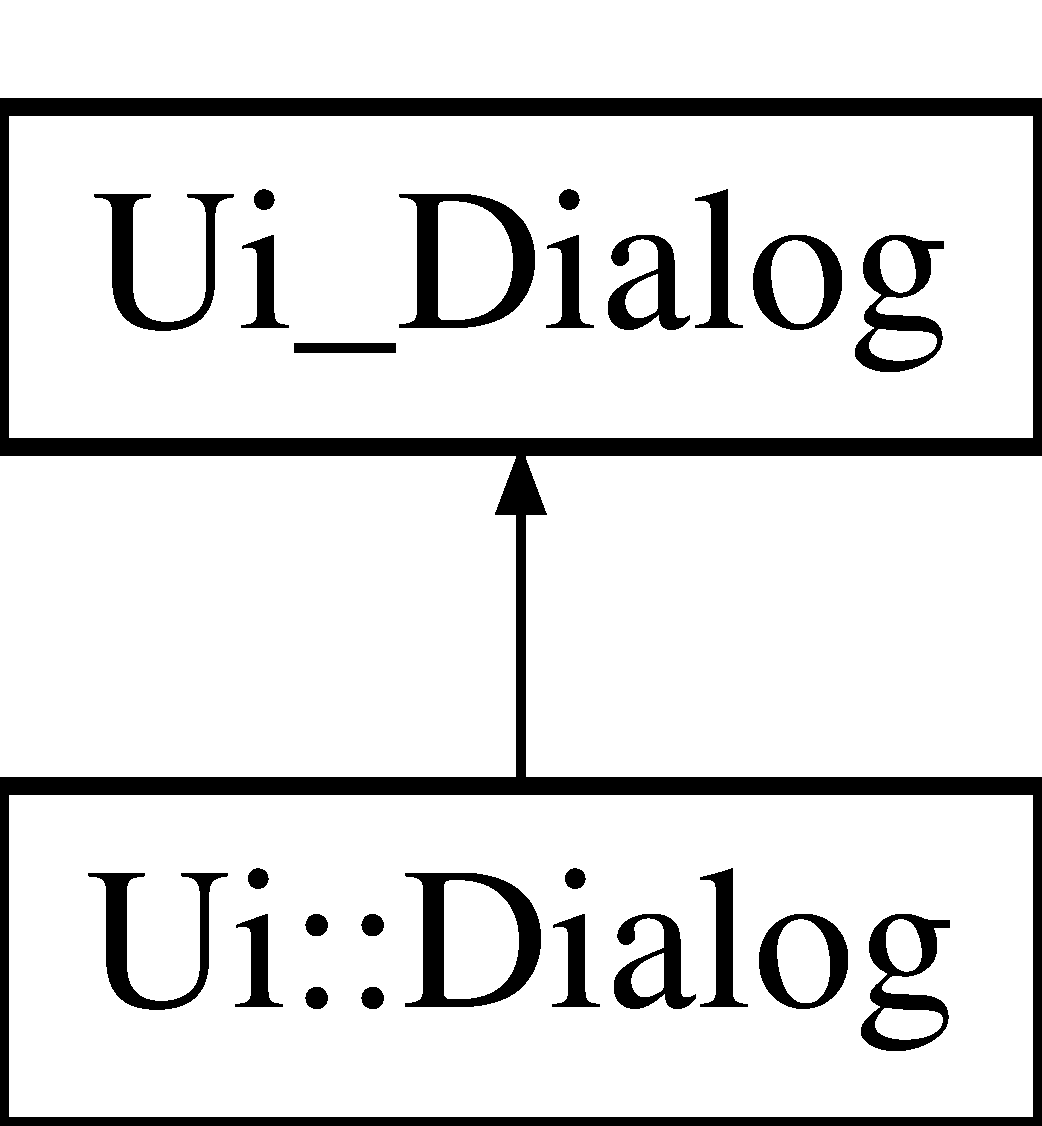
\includegraphics[height=2.000000cm]{classUi_1_1Dialog}
\end{center}
\end{figure}
\subsection*{Additional Inherited Members}


The documentation for this class was generated from the following file\-:\begin{DoxyCompactItemize}
\item 
ui\-\_\-dialog.\-h\end{DoxyCompactItemize}

\hypertarget{structFrame}{\section{Frame Struct Reference}
\label{structFrame}\index{Frame@{Frame}}
}
\subsection*{Public Member Functions}
\begin{DoxyCompactItemize}
\item 
\hypertarget{structFrame_a9964f5818030ca16524acb68c3355696}{{\bfseries Frame} (unsigned long int frame\-Num\-A, unsigned int player\-\_\-id\-A, double xpos\-A, double ypos\-A)}\label{structFrame_a9964f5818030ca16524acb68c3355696}

\item 
\hypertarget{structFrame_a9964f5818030ca16524acb68c3355696}{{\bfseries Frame} (unsigned long int frame\-Num\-A, unsigned int player\-\_\-id\-A, double xpos\-A, double ypos\-A)}\label{structFrame_a9964f5818030ca16524acb68c3355696}

\end{DoxyCompactItemize}
\subsection*{Public Attributes}
\begin{DoxyCompactItemize}
\item 
\hypertarget{structFrame_a6e2a3b730bf084aa6e59acf9fc7cab45}{unsigned long int {\bfseries frame\-Num}}\label{structFrame_a6e2a3b730bf084aa6e59acf9fc7cab45}

\item 
\hypertarget{structFrame_a7f7492c8ed7d6e932fe1161d04d73f2d}{unsigned int {\bfseries player\-\_\-id}}\label{structFrame_a7f7492c8ed7d6e932fe1161d04d73f2d}

\item 
\hypertarget{structFrame_a695df9509f1f1e67e3a1dbe45aec247c}{double {\bfseries xpos}}\label{structFrame_a695df9509f1f1e67e3a1dbe45aec247c}

\item 
\hypertarget{structFrame_ae37df21b384dd84305dfeea5bb60cfd5}{double {\bfseries ypos}}\label{structFrame_ae37df21b384dd84305dfeea5bb60cfd5}

\end{DoxyCompactItemize}


The documentation for this struct was generated from the following files\-:\begin{DoxyCompactItemize}
\item 
aceval.\-h\item 
dbthread.\-h\end{DoxyCompactItemize}

\hypertarget{classUi_1_1NewDB}{\section{Ui\-:\-:New\-D\-B Class Reference}
\label{classUi_1_1NewDB}\index{Ui\-::\-New\-D\-B@{Ui\-::\-New\-D\-B}}
}
Inheritance diagram for Ui\-:\-:New\-D\-B\-:\begin{figure}[H]
\begin{center}
\leavevmode
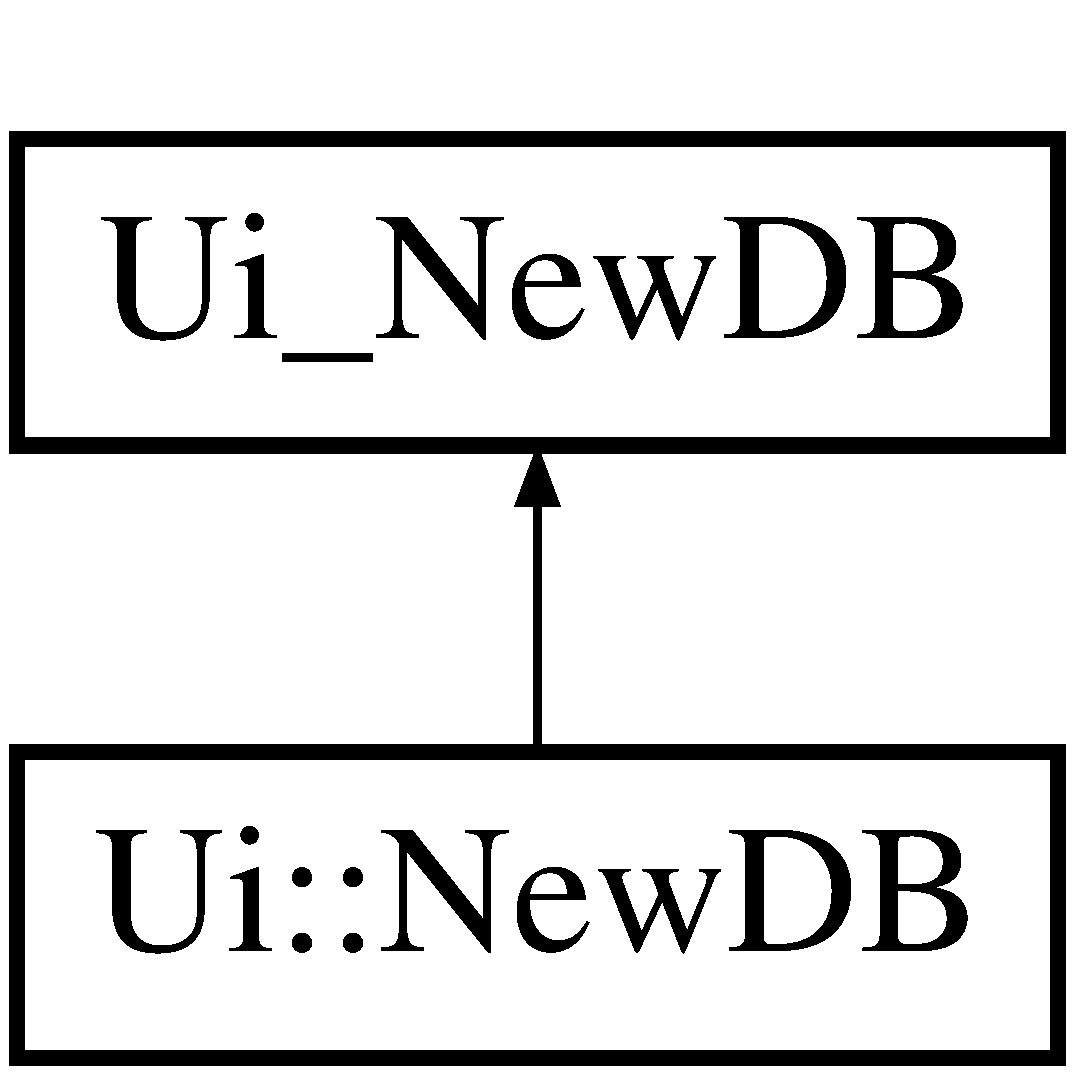
\includegraphics[height=2.000000cm]{classUi_1_1NewDB}
\end{center}
\end{figure}
\subsection*{Additional Inherited Members}


The documentation for this class was generated from the following file\-:\begin{DoxyCompactItemize}
\item 
ui\-\_\-newdb.\-h\end{DoxyCompactItemize}

\hypertarget{classNewDB}{\section{New\-D\-B Class Reference}
\label{classNewDB}\index{New\-D\-B@{New\-D\-B}}
}
\subsection*{Public Member Functions}
\begin{DoxyCompactItemize}
\item 
\hyperlink{classNewDB_a90318aa23cfbd4830348df1a4d9888d6}{New\-D\-B} (Q\-Widget $\ast$parent=0)
\begin{DoxyCompactList}\small\item\em \hyperlink{classNewDB_a90318aa23cfbd4830348df1a4d9888d6}{New\-D\-B\-::\-New\-D\-B}. \end{DoxyCompactList}\item 
\hyperlink{classNewDB_ad191442bdb36ad005acd2537482d9786}{$\sim$\-New\-D\-B} ()
\begin{DoxyCompactList}\small\item\em \hyperlink{classNewDB_ad191442bdb36ad005acd2537482d9786}{New\-D\-B\-::$\sim$\-New\-D\-B}. \end{DoxyCompactList}\item 
Q\-String \hyperlink{classNewDB_ad8c4702d2d4b9807eca620e4ed4327e4}{get\-Home} ()
\begin{DoxyCompactList}\small\item\em \hyperlink{classNewDB_ad8c4702d2d4b9807eca620e4ed4327e4}{New\-D\-B\-::get\-Home}. \end{DoxyCompactList}\item 
Q\-String \hyperlink{classNewDB_ac03466849c4a73c91856dfe08c28b1e0}{get\-Away} ()
\begin{DoxyCompactList}\small\item\em \hyperlink{classNewDB_ac03466849c4a73c91856dfe08c28b1e0}{New\-D\-B\-::get\-Away}. \end{DoxyCompactList}\item 
Q\-String \hyperlink{classNewDB_ad630fe28801a02211b4e72f3b3b624f8}{get\-Day} ()
\begin{DoxyCompactList}\small\item\em \hyperlink{classNewDB_ad630fe28801a02211b4e72f3b3b624f8}{New\-D\-B\-::get\-Day}. \end{DoxyCompactList}\item 
Q\-String \hyperlink{classNewDB_a697a2084248738f1b865db3987963c87}{get\-Month} ()
\begin{DoxyCompactList}\small\item\em \hyperlink{classNewDB_a697a2084248738f1b865db3987963c87}{New\-D\-B\-::get\-Month}. \end{DoxyCompactList}\item 
Q\-String \hyperlink{classNewDB_aea2a694c34450d05fa1b500439fd10f3}{get\-Year} ()
\begin{DoxyCompactList}\small\item\em \hyperlink{classNewDB_aea2a694c34450d05fa1b500439fd10f3}{New\-D\-B\-::get\-Year}. \end{DoxyCompactList}\end{DoxyCompactItemize}


\subsection{Constructor \& Destructor Documentation}
\hypertarget{classNewDB_a90318aa23cfbd4830348df1a4d9888d6}{\index{New\-D\-B@{New\-D\-B}!New\-D\-B@{New\-D\-B}}
\index{New\-D\-B@{New\-D\-B}!NewDB@{New\-D\-B}}
\subsubsection[{New\-D\-B}]{\setlength{\rightskip}{0pt plus 5cm}New\-D\-B\-::\-New\-D\-B (
\begin{DoxyParamCaption}
\item[{Q\-Widget $\ast$}]{parent = {\ttfamily 0}}
\end{DoxyParamCaption}
)\hspace{0.3cm}{\ttfamily [explicit]}}}\label{classNewDB_a90318aa23cfbd4830348df1a4d9888d6}


\hyperlink{classNewDB_a90318aa23cfbd4830348df1a4d9888d6}{New\-D\-B\-::\-New\-D\-B}. 


\begin{DoxyParams}{Parameters}
{\em parent} & Constructor for initializing the new db dialog \\
\hline
\end{DoxyParams}
\hypertarget{classNewDB_ad191442bdb36ad005acd2537482d9786}{\index{New\-D\-B@{New\-D\-B}!$\sim$\-New\-D\-B@{$\sim$\-New\-D\-B}}
\index{$\sim$\-New\-D\-B@{$\sim$\-New\-D\-B}!NewDB@{New\-D\-B}}
\subsubsection[{$\sim$\-New\-D\-B}]{\setlength{\rightskip}{0pt plus 5cm}New\-D\-B\-::$\sim$\-New\-D\-B (
\begin{DoxyParamCaption}
{}
\end{DoxyParamCaption}
)}}\label{classNewDB_ad191442bdb36ad005acd2537482d9786}


\hyperlink{classNewDB_ad191442bdb36ad005acd2537482d9786}{New\-D\-B\-::$\sim$\-New\-D\-B}. 

Destructor for the New\-Db dialog created by qt 

\subsection{Member Function Documentation}
\hypertarget{classNewDB_ac03466849c4a73c91856dfe08c28b1e0}{\index{New\-D\-B@{New\-D\-B}!get\-Away@{get\-Away}}
\index{get\-Away@{get\-Away}!NewDB@{New\-D\-B}}
\subsubsection[{get\-Away}]{\setlength{\rightskip}{0pt plus 5cm}Q\-String New\-D\-B\-::get\-Away (
\begin{DoxyParamCaption}
{}
\end{DoxyParamCaption}
)}}\label{classNewDB_ac03466849c4a73c91856dfe08c28b1e0}


\hyperlink{classNewDB_ac03466849c4a73c91856dfe08c28b1e0}{New\-D\-B\-::get\-Away}. 

\begin{DoxyReturn}{Returns}
Name of the visitor team
\end{DoxyReturn}
Function to access the name of the visitor team \hypertarget{classNewDB_ad630fe28801a02211b4e72f3b3b624f8}{\index{New\-D\-B@{New\-D\-B}!get\-Day@{get\-Day}}
\index{get\-Day@{get\-Day}!NewDB@{New\-D\-B}}
\subsubsection[{get\-Day}]{\setlength{\rightskip}{0pt plus 5cm}Q\-String New\-D\-B\-::get\-Day (
\begin{DoxyParamCaption}
{}
\end{DoxyParamCaption}
)}}\label{classNewDB_ad630fe28801a02211b4e72f3b3b624f8}


\hyperlink{classNewDB_ad630fe28801a02211b4e72f3b3b624f8}{New\-D\-B\-::get\-Day}. 

\begin{DoxyReturn}{Returns}
Day of the match Function to access the day number of the match 
\end{DoxyReturn}
\hypertarget{classNewDB_ad8c4702d2d4b9807eca620e4ed4327e4}{\index{New\-D\-B@{New\-D\-B}!get\-Home@{get\-Home}}
\index{get\-Home@{get\-Home}!NewDB@{New\-D\-B}}
\subsubsection[{get\-Home}]{\setlength{\rightskip}{0pt plus 5cm}Q\-String New\-D\-B\-::get\-Home (
\begin{DoxyParamCaption}
{}
\end{DoxyParamCaption}
)}}\label{classNewDB_ad8c4702d2d4b9807eca620e4ed4327e4}


\hyperlink{classNewDB_ad8c4702d2d4b9807eca620e4ed4327e4}{New\-D\-B\-::get\-Home}. 

\begin{DoxyReturn}{Returns}
Name of the Home team Function to access the name of the home team 
\end{DoxyReturn}
\hypertarget{classNewDB_a697a2084248738f1b865db3987963c87}{\index{New\-D\-B@{New\-D\-B}!get\-Month@{get\-Month}}
\index{get\-Month@{get\-Month}!NewDB@{New\-D\-B}}
\subsubsection[{get\-Month}]{\setlength{\rightskip}{0pt plus 5cm}Q\-String New\-D\-B\-::get\-Month (
\begin{DoxyParamCaption}
{}
\end{DoxyParamCaption}
)}}\label{classNewDB_a697a2084248738f1b865db3987963c87}


\hyperlink{classNewDB_a697a2084248738f1b865db3987963c87}{New\-D\-B\-::get\-Month}. 

\begin{DoxyReturn}{Returns}
Month of the match
\end{DoxyReturn}
Function to access the month number of the match \hypertarget{classNewDB_aea2a694c34450d05fa1b500439fd10f3}{\index{New\-D\-B@{New\-D\-B}!get\-Year@{get\-Year}}
\index{get\-Year@{get\-Year}!NewDB@{New\-D\-B}}
\subsubsection[{get\-Year}]{\setlength{\rightskip}{0pt plus 5cm}Q\-String New\-D\-B\-::get\-Year (
\begin{DoxyParamCaption}
{}
\end{DoxyParamCaption}
)}}\label{classNewDB_aea2a694c34450d05fa1b500439fd10f3}


\hyperlink{classNewDB_aea2a694c34450d05fa1b500439fd10f3}{New\-D\-B\-::get\-Year}. 

\begin{DoxyReturn}{Returns}
The year
\end{DoxyReturn}
Function to access the year in which the match was carried out 

The documentation for this class was generated from the following files\-:\begin{DoxyCompactItemize}
\item 
newdb.\-h\item 
newdb.\-cpp\end{DoxyCompactItemize}

\hypertarget{classpipeline}{\section{pipeline Class Reference}
\label{classpipeline}\index{pipeline@{pipeline}}
}
\subsection*{Public Member Functions}
\begin{DoxyCompactItemize}
\item 
\hyperlink{classpipeline_a6b3597bc480ffca8b2350bf1e7f8afe5}{pipeline} (unsigned long Win\-I\-D, const char $\ast$Filename)
\begin{DoxyCompactList}\small\item\em \hyperlink{classpipeline_a6b3597bc480ffca8b2350bf1e7f8afe5}{pipeline\-::pipeline} \end{DoxyCompactList}\item 
\hypertarget{classpipeline_abcfd0f7d1563886f2f5539b528316092}{\hyperlink{classpipeline_abcfd0f7d1563886f2f5539b528316092}{$\sim$pipeline} ()}\label{classpipeline_abcfd0f7d1563886f2f5539b528316092}

\begin{DoxyCompactList}\small\item\em \hyperlink{classpipeline_abcfd0f7d1563886f2f5539b528316092}{pipeline\-::$\sim$pipeline} \end{DoxyCompactList}\item 
\hypertarget{classpipeline_adb5054fb6710d8d3140c4620cb4e1a73}{void \hyperlink{classpipeline_adb5054fb6710d8d3140c4620cb4e1a73}{Set\-Playing} (void)}\label{classpipeline_adb5054fb6710d8d3140c4620cb4e1a73}

\begin{DoxyCompactList}\small\item\em \hyperlink{classpipeline_adb5054fb6710d8d3140c4620cb4e1a73}{pipeline\-::\-Set\-Playing} Sets the Pipeline to playing. \end{DoxyCompactList}\item 
void \hyperlink{classpipeline_a938a4d81ca42711464a835849099c473}{Set\-Paused} (void)
\begin{DoxyCompactList}\small\item\em \hyperlink{classpipeline_a938a4d81ca42711464a835849099c473}{pipeline\-::\-Set\-Paused} \end{DoxyCompactList}\item 
\hypertarget{classpipeline_a2d491af7f94ea87a4495b861a8a121fb}{void \hyperlink{classpipeline_a2d491af7f94ea87a4495b861a8a121fb}{Set\-Null} (void)}\label{classpipeline_a2d491af7f94ea87a4495b861a8a121fb}

\begin{DoxyCompactList}\small\item\em \hyperlink{classpipeline_a2d491af7f94ea87a4495b861a8a121fb}{pipeline\-::\-Set\-Null} Sets the pipeline to null state \end{DoxyCompactList}\item 
double \hyperlink{classpipeline_a4ff30decc13a3f67af289cd3b0188407}{Get\-Duration} (void)
\begin{DoxyCompactList}\small\item\em \hyperlink{classpipeline_a4ff30decc13a3f67af289cd3b0188407}{pipeline\-::\-Get\-Duration} \end{DoxyCompactList}\item 
double \hyperlink{classpipeline_ab99b8798b7845fd6bc5193fa75658fa7}{Get\-Position} (void)
\begin{DoxyCompactList}\small\item\em \hyperlink{classpipeline_ab99b8798b7845fd6bc5193fa75658fa7}{pipeline\-::\-Get\-Position} \end{DoxyCompactList}\item 
void \hyperlink{classpipeline_a4f5b575f03f87f6cd83049fdbd3c7f63}{Change\-Speed} (int value)
\begin{DoxyCompactList}\small\item\em \hyperlink{classpipeline_a4f5b575f03f87f6cd83049fdbd3c7f63}{pipeline\-::\-Change\-Speed} \end{DoxyCompactList}\item 
\hypertarget{classpipeline_a429bdada0ac1649898216eb3f2e162e4}{void \hyperlink{classpipeline_a429bdada0ac1649898216eb3f2e162e4}{Prove\-Method} ()}\label{classpipeline_a429bdada0ac1649898216eb3f2e162e4}

\begin{DoxyCompactList}\small\item\em \hyperlink{classpipeline_a429bdada0ac1649898216eb3f2e162e4}{pipeline\-::\-Prove\-Method} Gets the framerate of the video. \end{DoxyCompactList}\end{DoxyCompactItemize}
\subsection*{Public Attributes}
\begin{DoxyCompactItemize}
\item 
\hypertarget{classpipeline_aa89a110362294fc2dd12f48b19e20117}{int {\bfseries Frame\-Rate\-\_\-\-Den}}\label{classpipeline_aa89a110362294fc2dd12f48b19e20117}

\item 
\hypertarget{classpipeline_aa36b45729ff2aa2ad09a141532e87f54}{int {\bfseries Frame\-Rate\-\_\-\-Num}}\label{classpipeline_aa36b45729ff2aa2ad09a141532e87f54}

\end{DoxyCompactItemize}


\subsection{Constructor \& Destructor Documentation}
\hypertarget{classpipeline_a6b3597bc480ffca8b2350bf1e7f8afe5}{\index{pipeline@{pipeline}!pipeline@{pipeline}}
\index{pipeline@{pipeline}!pipeline@{pipeline}}
\subsubsection[{pipeline}]{\setlength{\rightskip}{0pt plus 5cm}pipeline\-::pipeline (
\begin{DoxyParamCaption}
\item[{unsigned long}]{Win\-I\-D, }
\item[{const char $\ast$}]{Filename}
\end{DoxyParamCaption}
)}}\label{classpipeline_a6b3597bc480ffca8b2350bf1e7f8afe5}


\hyperlink{classpipeline_a6b3597bc480ffca8b2350bf1e7f8afe5}{pipeline\-::pipeline} 


\begin{DoxyParams}{Parameters}
{\em Win\-I\-D} & \\
\hline
{\em Filename} & Constructor for the Pipeline, generates all the elements and links them together to form the pipeline \\
\hline
\end{DoxyParams}


\subsection{Member Function Documentation}
\hypertarget{classpipeline_a4f5b575f03f87f6cd83049fdbd3c7f63}{\index{pipeline@{pipeline}!Change\-Speed@{Change\-Speed}}
\index{Change\-Speed@{Change\-Speed}!pipeline@{pipeline}}
\subsubsection[{Change\-Speed}]{\setlength{\rightskip}{0pt plus 5cm}void pipeline\-::\-Change\-Speed (
\begin{DoxyParamCaption}
\item[{int}]{value}
\end{DoxyParamCaption}
)}}\label{classpipeline_a4f5b575f03f87f6cd83049fdbd3c7f63}


\hyperlink{classpipeline_a4f5b575f03f87f6cd83049fdbd3c7f63}{pipeline\-::\-Change\-Speed} 


\begin{DoxyParams}{Parameters}
{\em value} & Changes the playback speed of the video. \\
\hline
\end{DoxyParams}
\hypertarget{classpipeline_a4ff30decc13a3f67af289cd3b0188407}{\index{pipeline@{pipeline}!Get\-Duration@{Get\-Duration}}
\index{Get\-Duration@{Get\-Duration}!pipeline@{pipeline}}
\subsubsection[{Get\-Duration}]{\setlength{\rightskip}{0pt plus 5cm}double pipeline\-::\-Get\-Duration (
\begin{DoxyParamCaption}
\item[{void}]{}
\end{DoxyParamCaption}
)}}\label{classpipeline_a4ff30decc13a3f67af289cd3b0188407}


\hyperlink{classpipeline_a4ff30decc13a3f67af289cd3b0188407}{pipeline\-::\-Get\-Duration} 

\begin{DoxyReturn}{Returns}
the duration of the video
\end{DoxyReturn}
Function to get the duration of a video. \hypertarget{classpipeline_ab99b8798b7845fd6bc5193fa75658fa7}{\index{pipeline@{pipeline}!Get\-Position@{Get\-Position}}
\index{Get\-Position@{Get\-Position}!pipeline@{pipeline}}
\subsubsection[{Get\-Position}]{\setlength{\rightskip}{0pt plus 5cm}double pipeline\-::\-Get\-Position (
\begin{DoxyParamCaption}
\item[{void}]{}
\end{DoxyParamCaption}
)}}\label{classpipeline_ab99b8798b7845fd6bc5193fa75658fa7}


\hyperlink{classpipeline_ab99b8798b7845fd6bc5193fa75658fa7}{pipeline\-::\-Get\-Position} 

\begin{DoxyReturn}{Returns}
the current time position of the video.
\end{DoxyReturn}
Returns the current position of the video. \hypertarget{classpipeline_a938a4d81ca42711464a835849099c473}{\index{pipeline@{pipeline}!Set\-Paused@{Set\-Paused}}
\index{Set\-Paused@{Set\-Paused}!pipeline@{pipeline}}
\subsubsection[{Set\-Paused}]{\setlength{\rightskip}{0pt plus 5cm}void pipeline\-::\-Set\-Paused (
\begin{DoxyParamCaption}
\item[{void}]{}
\end{DoxyParamCaption}
)}}\label{classpipeline_a938a4d81ca42711464a835849099c473}


\hyperlink{classpipeline_a938a4d81ca42711464a835849099c473}{pipeline\-::\-Set\-Paused} 

Sets the pipeline to paused state. 

The documentation for this class was generated from the following files\-:\begin{DoxyCompactItemize}
\item 
pipeline.\-h\item 
pipeline.\-cpp\end{DoxyCompactItemize}

\hypertarget{classPlayer}{\section{Player Class Reference}
\label{classPlayer}\index{Player@{Player}}
}
\subsection*{Public Member Functions}
\begin{DoxyCompactItemize}
\item 
\hypertarget{classPlayer_a915010f972014f45848d1c211418ec42}{{\bfseries Player} (Q\-String Name\-\_\-\-Val, Q\-String Tag\-\_\-\-Val, int Number\-\_\-\-Val)}\label{classPlayer_a915010f972014f45848d1c211418ec42}

\item 
\hypertarget{classPlayer_a630f7472998f255377bb6bcb7b0e1932}{bool {\bfseries operator==} (const \hyperlink{classPlayer}{Player} \&player\-C) const }\label{classPlayer_a630f7472998f255377bb6bcb7b0e1932}

\end{DoxyCompactItemize}
\subsection*{Public Attributes}
\begin{DoxyCompactItemize}
\item 
\hypertarget{classPlayer_a9ffaa7b4cf8667a2a8de3e9cea51a8b5}{Q\-String {\bfseries Name}}\label{classPlayer_a9ffaa7b4cf8667a2a8de3e9cea51a8b5}

\item 
\hypertarget{classPlayer_ac55e5a1e2488281d11bc34d1141fda96}{Q\-String {\bfseries Tag}}\label{classPlayer_ac55e5a1e2488281d11bc34d1141fda96}

\item 
\hypertarget{classPlayer_a7152dbf1e4c28728e841f5b6a2ad755e}{int {\bfseries Number}}\label{classPlayer_a7152dbf1e4c28728e841f5b6a2ad755e}

\end{DoxyCompactItemize}


The documentation for this class was generated from the following file\-:\begin{DoxyCompactItemize}
\item 
player.\-h\end{DoxyCompactItemize}

\hypertarget{classPlayerDialog}{\section{Player\-Dialog Class Reference}
\label{classPlayerDialog}\index{Player\-Dialog@{Player\-Dialog}}
}
\subsection*{Public Member Functions}
\begin{DoxyCompactItemize}
\item 
\hypertarget{classPlayerDialog_a41ca59c1acdc2f3c1fc7657b0dab0175}{{\bfseries Player\-Dialog} (Q\-Widget $\ast$parent=0)}\label{classPlayerDialog_a41ca59c1acdc2f3c1fc7657b0dab0175}

\item 
\hypertarget{classPlayerDialog_a33050c9714b08b112f3d35640e66deba}{Q\-String {\bfseries Get\-Name} ()}\label{classPlayerDialog_a33050c9714b08b112f3d35640e66deba}

\item 
\hypertarget{classPlayerDialog_a475df1a0286dca259f8ecaf6d0f60f54}{Q\-String {\bfseries Get\-Num} ()}\label{classPlayerDialog_a475df1a0286dca259f8ecaf6d0f60f54}

\item 
\hypertarget{classPlayerDialog_aaf646807bb272755ce306732b5270a3c}{Q\-String {\bfseries Get\-Team} ()}\label{classPlayerDialog_aaf646807bb272755ce306732b5270a3c}

\end{DoxyCompactItemize}


The documentation for this class was generated from the following files\-:\begin{DoxyCompactItemize}
\item 
playerdialog.\-h\item 
playerdialog.\-cpp\end{DoxyCompactItemize}

\hypertarget{classUi_1_1PlayerDialog}{\section{Ui\-:\-:Player\-Dialog Class Reference}
\label{classUi_1_1PlayerDialog}\index{Ui\-::\-Player\-Dialog@{Ui\-::\-Player\-Dialog}}
}
Inheritance diagram for Ui\-:\-:Player\-Dialog\-:\begin{figure}[H]
\begin{center}
\leavevmode
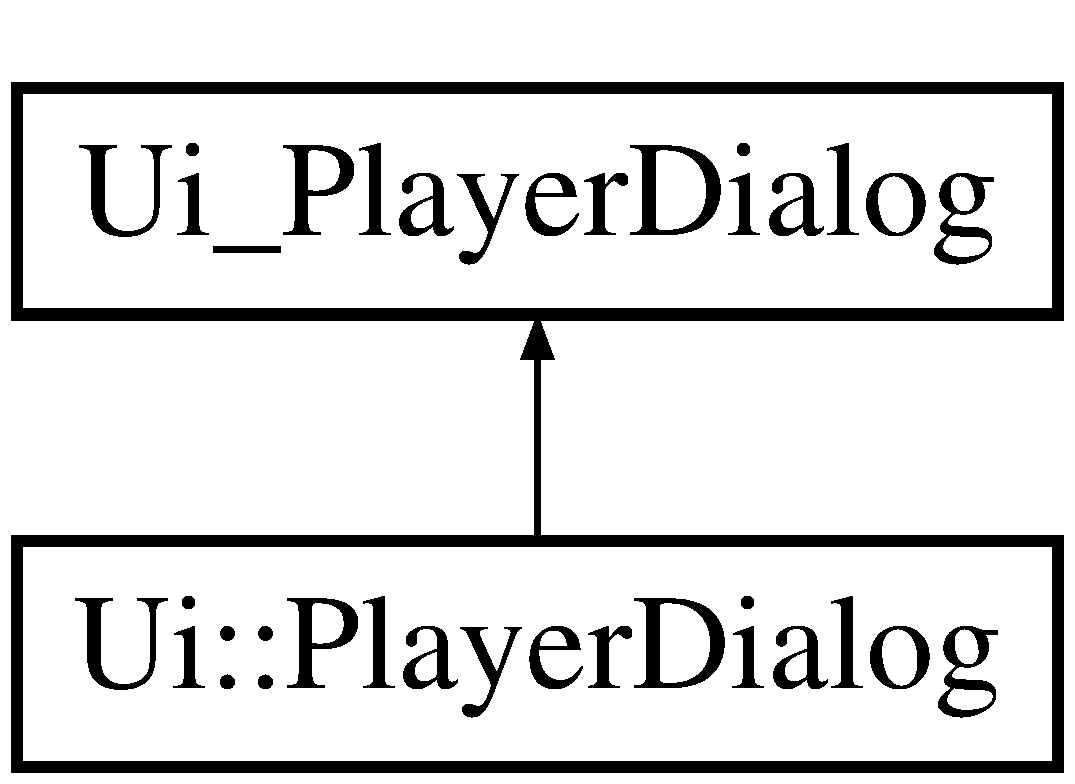
\includegraphics[height=2.000000cm]{classUi_1_1PlayerDialog}
\end{center}
\end{figure}
\subsection*{Additional Inherited Members}


The documentation for this class was generated from the following file\-:\begin{DoxyCompactItemize}
\item 
ui\-\_\-playerdialog.\-h\end{DoxyCompactItemize}

\hypertarget{classPlayersControl}{\section{Players\-Control Class Reference}
\label{classPlayersControl}\index{Players\-Control@{Players\-Control}}
}
\subsection*{Public Member Functions}
\begin{DoxyCompactItemize}
\item 
\hypertarget{classPlayersControl_a593957bc4333b43d2ed2188dca0e5e89}{{\bfseries Players\-Control} (Q\-Vector$<$ \hyperlink{classPlayer}{Player} $>$ \&, Q\-Widget $\ast$parent=0)}\label{classPlayersControl_a593957bc4333b43d2ed2188dca0e5e89}

\item 
\hypertarget{classPlayersControl_afb74e0c42d6a105aa1370a92b3af238a}{int {\bfseries get\-Row} ()}\label{classPlayersControl_afb74e0c42d6a105aa1370a92b3af238a}

\end{DoxyCompactItemize}


The documentation for this class was generated from the following files\-:\begin{DoxyCompactItemize}
\item 
playerscontrol.\-h\item 
playerscontrol.\-cpp\end{DoxyCompactItemize}

\hypertarget{classUi_1_1PlayersControl}{\section{Ui\-:\-:Players\-Control Class Reference}
\label{classUi_1_1PlayersControl}\index{Ui\-::\-Players\-Control@{Ui\-::\-Players\-Control}}
}
Inheritance diagram for Ui\-:\-:Players\-Control\-:\begin{figure}[H]
\begin{center}
\leavevmode
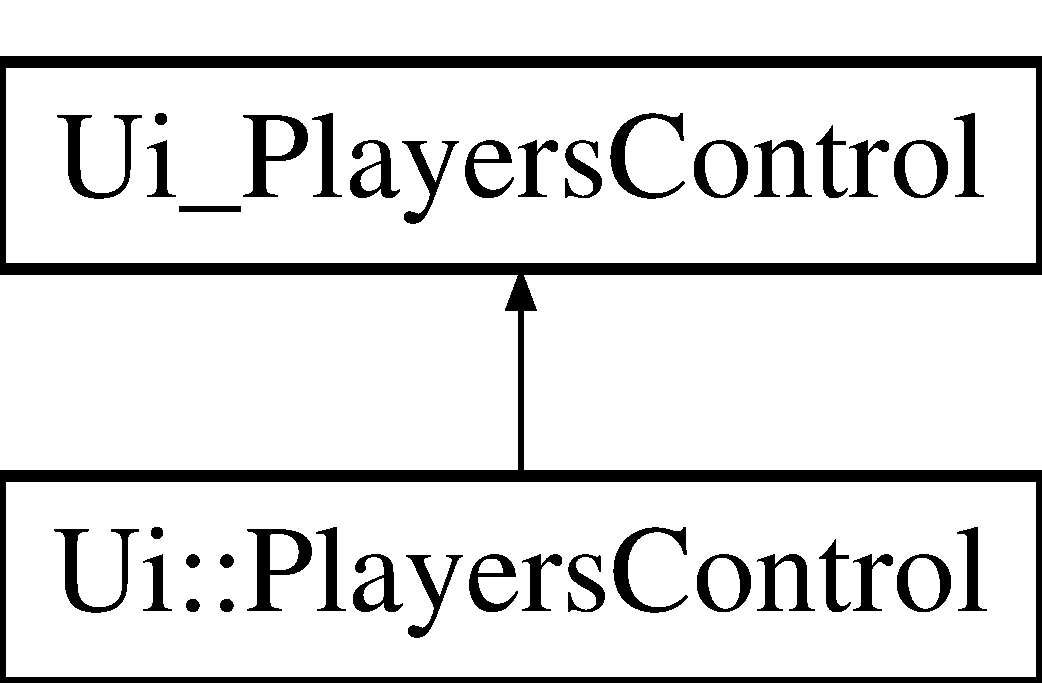
\includegraphics[height=2.000000cm]{classUi_1_1PlayersControl}
\end{center}
\end{figure}
\subsection*{Additional Inherited Members}


The documentation for this class was generated from the following file\-:\begin{DoxyCompactItemize}
\item 
ui\-\_\-playerscontrol.\-h\end{DoxyCompactItemize}

\hypertarget{classScene}{\section{Scene Class Reference}
\label{classScene}\index{Scene@{Scene}}
}
\subsection*{Public Member Functions}
\begin{DoxyCompactItemize}
\item 
\hypertarget{classScene_aaa81008f41154cc769e9bb7bcbd12848}{{\bfseries Scene} (double Fun\-Init\-Time, Q\-String Label\-Pa)}\label{classScene_aaa81008f41154cc769e9bb7bcbd12848}

\item 
\hypertarget{classScene_a2eff52baba0b72c10353d6eb955fae89}{void {\bfseries Add\-Player} (int \hyperlink{classPlayer}{Player})}\label{classScene_a2eff52baba0b72c10353d6eb955fae89}

\item 
\hypertarget{classScene_a1d53c932387315709caefce7dead7337}{double {\bfseries Get\-Init\-Time} ()}\label{classScene_a1d53c932387315709caefce7dead7337}

\item 
\hypertarget{classScene_a38ec70e43222865dd455ec5540a8f2ba}{double {\bfseries Get\-Fin\-Time} ()}\label{classScene_a38ec70e43222865dd455ec5540a8f2ba}

\item 
\hypertarget{classScene_a160577801115c5987b474af5fb6db6d0}{void {\bfseries Set\-Fin\-Time} (double Fun\-Fin\-Time)}\label{classScene_a160577801115c5987b474af5fb6db6d0}

\item 
\hypertarget{classScene_a61cc64b393317b62ee3734afe852a4f6}{Q\-String {\bfseries Get\-Label} () const }\label{classScene_a61cc64b393317b62ee3734afe852a4f6}

\end{DoxyCompactItemize}
\subsection*{Public Attributes}
\begin{DoxyCompactItemize}
\item 
\hypertarget{classScene_a407c1509f4bbddc027ea67bccc0e063a}{Q\-Vector$<$ int $>$ {\bfseries Players}}\label{classScene_a407c1509f4bbddc027ea67bccc0e063a}

\end{DoxyCompactItemize}


The documentation for this class was generated from the following file\-:\begin{DoxyCompactItemize}
\item 
scene.\-h\end{DoxyCompactItemize}

\hypertarget{classSceneDialog}{\section{Scene\-Dialog Class Reference}
\label{classSceneDialog}\index{Scene\-Dialog@{Scene\-Dialog}}
}
\subsection*{Public Member Functions}
\begin{DoxyCompactItemize}
\item 
\hypertarget{classSceneDialog_a48fbdf6f9f4080a23380655b416989ee}{{\bfseries Scene\-Dialog} (Q\-Widget $\ast$parent=0)}\label{classSceneDialog_a48fbdf6f9f4080a23380655b416989ee}

\item 
\hypertarget{classSceneDialog_aa9fd8578cfafda5d6ed73cb2e82ad64d}{Q\-String {\bfseries Get\-Label} ()}\label{classSceneDialog_aa9fd8578cfafda5d6ed73cb2e82ad64d}

\end{DoxyCompactItemize}


The documentation for this class was generated from the following files\-:\begin{DoxyCompactItemize}
\item 
scenedialog.\-h\item 
scenedialog.\-cpp\end{DoxyCompactItemize}

\hypertarget{classUi_1_1SceneDialog}{\section{Ui\-:\-:Scene\-Dialog Class Reference}
\label{classUi_1_1SceneDialog}\index{Ui\-::\-Scene\-Dialog@{Ui\-::\-Scene\-Dialog}}
}
Inheritance diagram for Ui\-:\-:Scene\-Dialog\-:\begin{figure}[H]
\begin{center}
\leavevmode
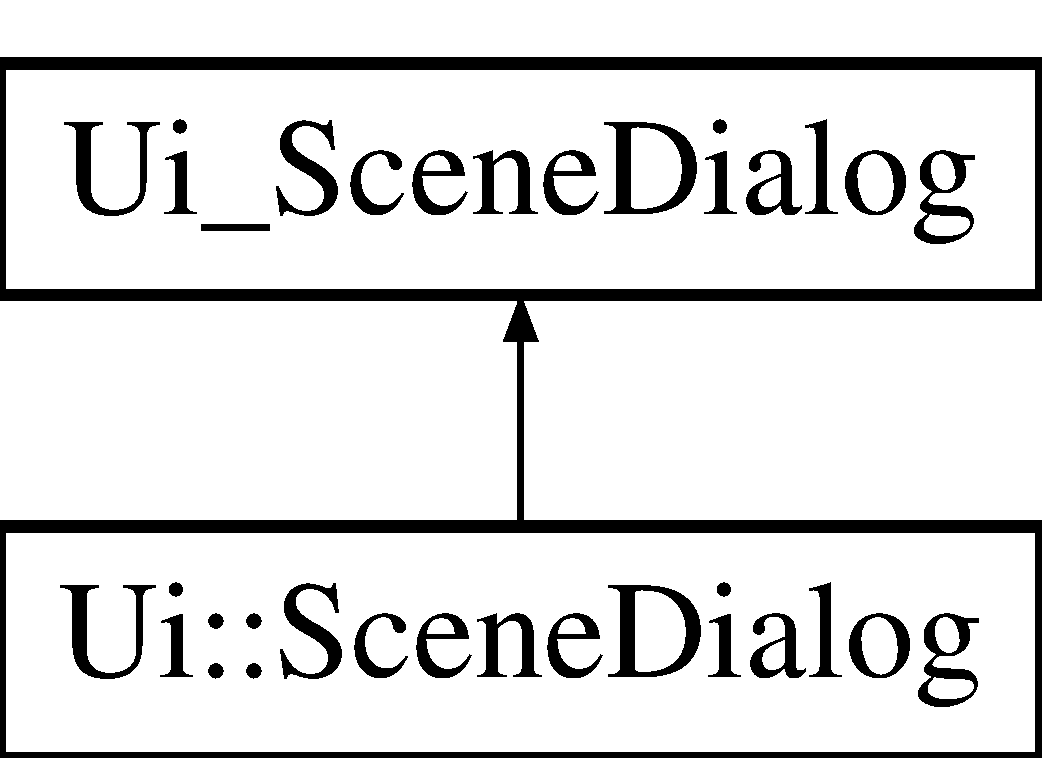
\includegraphics[height=2.000000cm]{classUi_1_1SceneDialog}
\end{center}
\end{figure}
\subsection*{Additional Inherited Members}


The documentation for this class was generated from the following file\-:\begin{DoxyCompactItemize}
\item 
ui\-\_\-scenedialog.\-h\end{DoxyCompactItemize}

\hypertarget{classUi__AceVal}{\section{Ui\-\_\-\-Ace\-Val Class Reference}
\label{classUi__AceVal}\index{Ui\-\_\-\-Ace\-Val@{Ui\-\_\-\-Ace\-Val}}
}
Inheritance diagram for Ui\-\_\-\-Ace\-Val\-:\begin{figure}[H]
\begin{center}
\leavevmode
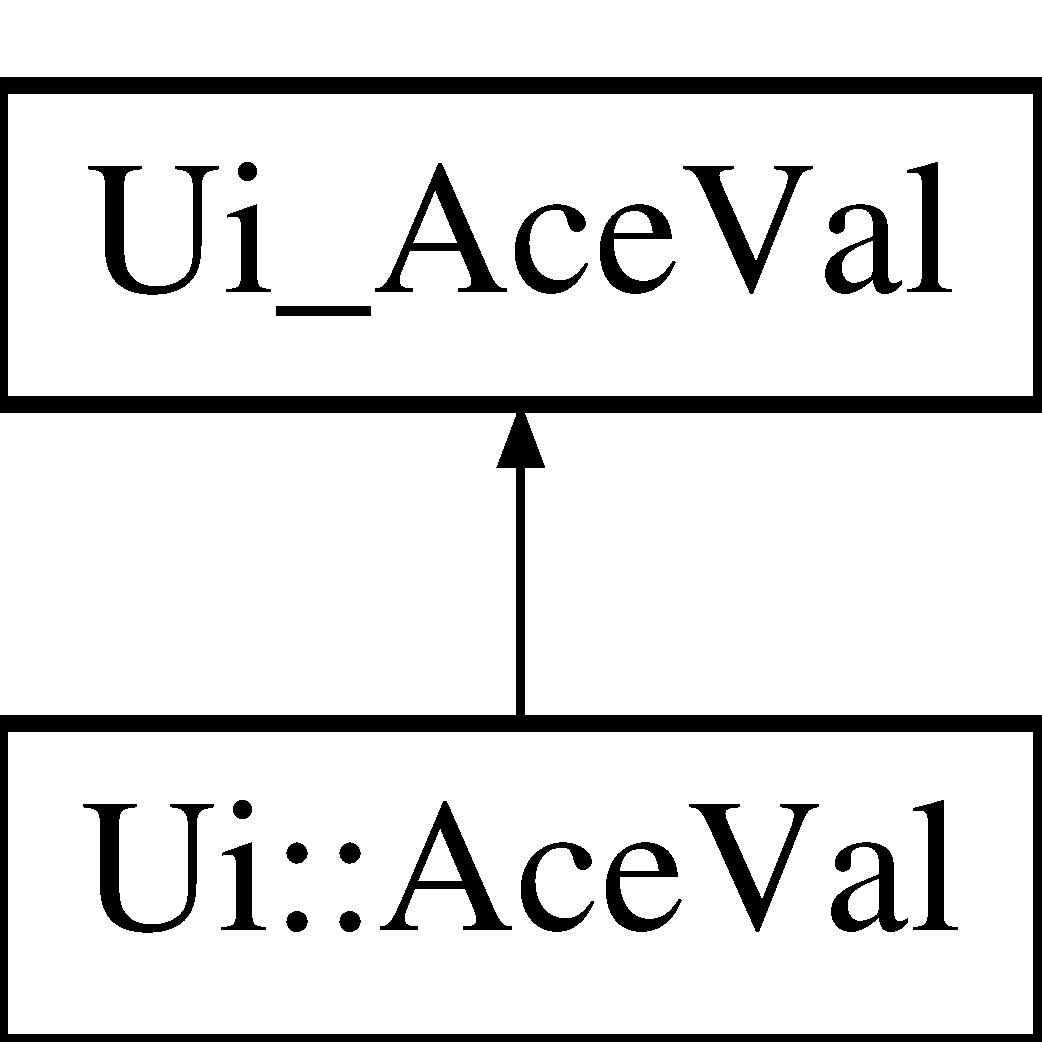
\includegraphics[height=2.000000cm]{classUi__AceVal}
\end{center}
\end{figure}
\subsection*{Public Member Functions}
\begin{DoxyCompactItemize}
\item 
\hypertarget{classUi__AceVal_a72f0d370e0d02783207d8dec4b1f9f11}{void {\bfseries setup\-Ui} (Q\-Main\-Window $\ast$\hyperlink{classAceVal}{Ace\-Val})}\label{classUi__AceVal_a72f0d370e0d02783207d8dec4b1f9f11}

\item 
\hypertarget{classUi__AceVal_a98089ae6994a12ccf66b540dde835b8e}{void {\bfseries retranslate\-Ui} (Q\-Main\-Window $\ast$\hyperlink{classAceVal}{Ace\-Val})}\label{classUi__AceVal_a98089ae6994a12ccf66b540dde835b8e}

\end{DoxyCompactItemize}
\subsection*{Public Attributes}
\begin{DoxyCompactItemize}
\item 
\hypertarget{classUi__AceVal_a30174a042540dce12d3de018215d14fc}{Q\-Action $\ast$ {\bfseries action\-Open\-\_\-\-File}}\label{classUi__AceVal_a30174a042540dce12d3de018215d14fc}

\item 
\hypertarget{classUi__AceVal_a0bee4d733dfb7131f173b0c10471e5ea}{Q\-Action $\ast$ {\bfseries action\-Save\-\_\-\-File}}\label{classUi__AceVal_a0bee4d733dfb7131f173b0c10471e5ea}

\item 
\hypertarget{classUi__AceVal_a09b7bc348529e4e1284a6f51b12437c9}{Q\-Action $\ast$ {\bfseries action\-Close}}\label{classUi__AceVal_a09b7bc348529e4e1284a6f51b12437c9}

\item 
\hypertarget{classUi__AceVal_ab640e572260888564ec9fe82e48c500c}{Q\-Action $\ast$ {\bfseries action\-Frame\-\_\-by\-\_\-frame}}\label{classUi__AceVal_ab640e572260888564ec9fe82e48c500c}

\item 
\hypertarget{classUi__AceVal_a3a2142b903d7235d4c7686fae0461a0a}{Q\-Action $\ast$ {\bfseries action\-Play}}\label{classUi__AceVal_a3a2142b903d7235d4c7686fae0461a0a}

\item 
\hypertarget{classUi__AceVal_a766e2d4b27f3ef553fc202ad083c7488}{Q\-Action $\ast$ {\bfseries action\-Pause}}\label{classUi__AceVal_a766e2d4b27f3ef553fc202ad083c7488}

\item 
\hypertarget{classUi__AceVal_af71bf918dd405ef5986f164da7c3b7bf}{Q\-Action $\ast$ {\bfseries action\-Stop}}\label{classUi__AceVal_af71bf918dd405ef5986f164da7c3b7bf}

\item 
\hypertarget{classUi__AceVal_a76ec53c1bca70bd211add11284b04a87}{Q\-Action $\ast$ {\bfseries action\-Properties}}\label{classUi__AceVal_a76ec53c1bca70bd211add11284b04a87}

\item 
\hypertarget{classUi__AceVal_ad090150db9686388f1e0ab95a4f8c9d5}{Q\-Action $\ast$ {\bfseries action\-Insert\-\_\-\-Player}}\label{classUi__AceVal_ad090150db9686388f1e0ab95a4f8c9d5}

\item 
\hypertarget{classUi__AceVal_a2a2b8ceead337432a6237a3723eb60b7}{Q\-Action $\ast$ {\bfseries action\-Insert\-\_\-\-Scene}}\label{classUi__AceVal_a2a2b8ceead337432a6237a3723eb60b7}

\item 
\hypertarget{classUi__AceVal_a64e0ac58c359a39e4a5b5de19e4891f7}{Q\-Action $\ast$ {\bfseries action\-Scenes\-\_\-\-List}}\label{classUi__AceVal_a64e0ac58c359a39e4a5b5de19e4891f7}

\item 
\hypertarget{classUi__AceVal_a4788d12d921a9714f1ca210434c5368a}{Q\-Action $\ast$ {\bfseries action\-Home}}\label{classUi__AceVal_a4788d12d921a9714f1ca210434c5368a}

\item 
\hypertarget{classUi__AceVal_ae0aa321f967de4dc3394751141e4278b}{Q\-Action $\ast$ {\bfseries action\-Away}}\label{classUi__AceVal_ae0aa321f967de4dc3394751141e4278b}

\item 
\hypertarget{classUi__AceVal_a5ba1a5d61bb5c2b09c7a2dbb26a28ff1}{Q\-Action $\ast$ {\bfseries action\-Connect}}\label{classUi__AceVal_a5ba1a5d61bb5c2b09c7a2dbb26a28ff1}

\item 
\hypertarget{classUi__AceVal_a22d1cec32bd2d6dbb76936bd8f90752e}{Q\-Action $\ast$ {\bfseries action\-My\-S\-Q\-L}}\label{classUi__AceVal_a22d1cec32bd2d6dbb76936bd8f90752e}

\item 
\hypertarget{classUi__AceVal_a87bc409615c182caa9b8a0d479faebb1}{Q\-Action $\ast$ {\bfseries action\-Y\-A\-M\-L}}\label{classUi__AceVal_a87bc409615c182caa9b8a0d479faebb1}

\item 
\hypertarget{classUi__AceVal_a92b0e8f846d5e678af31a61e02255a3e}{Q\-Action $\ast$ {\bfseries action\-Open\-\_\-\-D\-B}}\label{classUi__AceVal_a92b0e8f846d5e678af31a61e02255a3e}

\item 
\hypertarget{classUi__AceVal_af190d26af039b584178dba507f4bb172}{Q\-Action $\ast$ {\bfseries action\-New\-\_\-\-D\-B}}\label{classUi__AceVal_af190d26af039b584178dba507f4bb172}

\item 
\hypertarget{classUi__AceVal_a92b3be5e4d9dd6c31a9330c84be4b26a}{Q\-Action $\ast$ {\bfseries action\-Activate}}\label{classUi__AceVal_a92b3be5e4d9dd6c31a9330c84be4b26a}

\item 
\hypertarget{classUi__AceVal_a2400795137f7a7e3e9ac2d2d00c29d62}{Q\-Action $\ast$ {\bfseries action\-Select\-\_\-\-Player}}\label{classUi__AceVal_a2400795137f7a7e3e9ac2d2d00c29d62}

\item 
\hypertarget{classUi__AceVal_ae3939fb48e886edcc57f03276f23ecb5}{Q\-Widget $\ast$ {\bfseries central\-Widget}}\label{classUi__AceVal_ae3939fb48e886edcc57f03276f23ecb5}

\item 
\hypertarget{classUi__AceVal_a66bc27f323d406bd1bf3cd1a6338232e}{Q\-V\-Box\-Layout $\ast$ {\bfseries vertical\-Layout\-\_\-10}}\label{classUi__AceVal_a66bc27f323d406bd1bf3cd1a6338232e}

\item 
\hypertarget{classUi__AceVal_ac60d78636d21b91bc881c1ee3c6ff280}{Q\-H\-Box\-Layout $\ast$ {\bfseries horizontal\-Layout\-\_\-5}}\label{classUi__AceVal_ac60d78636d21b91bc881c1ee3c6ff280}

\item 
\hypertarget{classUi__AceVal_a348df195ff78fabecaa6ee6347e37f45}{Q\-Frame $\ast$ {\bfseries frame\-\_\-7}}\label{classUi__AceVal_a348df195ff78fabecaa6ee6347e37f45}

\item 
\hypertarget{classUi__AceVal_a3ab0b4f9b6f1e01e1668c91b5d0133db}{Q\-V\-Box\-Layout $\ast$ {\bfseries vertical\-Layout\-\_\-5}}\label{classUi__AceVal_a3ab0b4f9b6f1e01e1668c91b5d0133db}

\item 
\hypertarget{classUi__AceVal_a0c72362206fe5ae1af91d0d9c6b0a23a}{Q\-Frame $\ast$ {\bfseries line\-\_\-2}}\label{classUi__AceVal_a0c72362206fe5ae1af91d0d9c6b0a23a}

\item 
\hypertarget{classUi__AceVal_a35ea372d3661022d304690597fafd9d2}{Q\-H\-Box\-Layout $\ast$ {\bfseries horizontal\-Layout\-\_\-8}}\label{classUi__AceVal_a35ea372d3661022d304690597fafd9d2}

\item 
\hypertarget{classUi__AceVal_a53e31621fcad9282ba88405843fb8707}{Q\-V\-Box\-Layout $\ast$ {\bfseries vertical\-Layout\-\_\-9}}\label{classUi__AceVal_a53e31621fcad9282ba88405843fb8707}

\item 
\hypertarget{classUi__AceVal_a7a10dfd0528c80e84cf72ead7cefeeae}{Q\-H\-Box\-Layout $\ast$ {\bfseries horizontal\-Layout\-\_\-6}}\label{classUi__AceVal_a7a10dfd0528c80e84cf72ead7cefeeae}

\item 
\hypertarget{classUi__AceVal_aa2cfd5ea2d279fd8b45485551d72bdc2}{Q\-V\-Box\-Layout $\ast$ {\bfseries vertical\-Layout\-\_\-7}}\label{classUi__AceVal_aa2cfd5ea2d279fd8b45485551d72bdc2}

\item 
\hypertarget{classUi__AceVal_a3856cc794d426d5209fbc379e22f8ebb}{Q\-Label $\ast$ {\bfseries label\-\_\-11}}\label{classUi__AceVal_a3856cc794d426d5209fbc379e22f8ebb}

\item 
\hypertarget{classUi__AceVal_a474baa92647cd1bce1dfeb274294a178}{Q\-Label $\ast$ {\bfseries label\-\_\-12}}\label{classUi__AceVal_a474baa92647cd1bce1dfeb274294a178}

\item 
\hypertarget{classUi__AceVal_a563da3e5963fb36ce97a1968599c1758}{Q\-V\-Box\-Layout $\ast$ {\bfseries vertical\-Layout\-\_\-8}}\label{classUi__AceVal_a563da3e5963fb36ce97a1968599c1758}

\item 
\hypertarget{classUi__AceVal_a9b59b8a8aca8b07b62a44ec2405b9e68}{Q\-Slider $\ast$ {\bfseries horizontal\-Slider}}\label{classUi__AceVal_a9b59b8a8aca8b07b62a44ec2405b9e68}

\item 
\hypertarget{classUi__AceVal_ad0966ef3ffbc3d8398525a33c43f65d1}{Q\-Spin\-Box $\ast$ {\bfseries spin\-Box\-\_\-2}}\label{classUi__AceVal_ad0966ef3ffbc3d8398525a33c43f65d1}

\item 
\hypertarget{classUi__AceVal_a46d39ba7f5091f2dc86d7299d71f539f}{Q\-H\-Box\-Layout $\ast$ {\bfseries horizontal\-Layout\-\_\-7}}\label{classUi__AceVal_a46d39ba7f5091f2dc86d7299d71f539f}

\item 
\hypertarget{classUi__AceVal_a68cbb449653b1c67299f8f17e5d5e02e}{Q\-Spacer\-Item $\ast$ {\bfseries horizontal\-Spacer}}\label{classUi__AceVal_a68cbb449653b1c67299f8f17e5d5e02e}

\item 
\hypertarget{classUi__AceVal_ae9f7fdf2f30dadf032987d442c502086}{Q\-Tool\-Button $\ast$ {\bfseries tool\-Button\-\_\-3}}\label{classUi__AceVal_ae9f7fdf2f30dadf032987d442c502086}

\item 
\hypertarget{classUi__AceVal_adeefacee7f1f83033877caa9d475b65e}{Q\-Tool\-Button $\ast$ {\bfseries tool\-Button\-\_\-4}}\label{classUi__AceVal_adeefacee7f1f83033877caa9d475b65e}

\item 
\hypertarget{classUi__AceVal_aba668413e829998ba4b29269b41194f2}{Q\-Tool\-Button $\ast$ {\bfseries tool\-Button\-\_\-5}}\label{classUi__AceVal_aba668413e829998ba4b29269b41194f2}

\item 
\hypertarget{classUi__AceVal_a85120a44ccdf8c5529a193f56bb59671}{Q\-Spacer\-Item $\ast$ {\bfseries horizontal\-Spacer\-\_\-2}}\label{classUi__AceVal_a85120a44ccdf8c5529a193f56bb59671}

\item 
\hypertarget{classUi__AceVal_a7ead7f0196975fdbfb7b5a7733d103f7}{Q\-Menu\-Bar $\ast$ {\bfseries menu\-Bar}}\label{classUi__AceVal_a7ead7f0196975fdbfb7b5a7733d103f7}

\item 
\hypertarget{classUi__AceVal_ac19d54ca34529a87a48184c69968ad43}{Q\-Menu $\ast$ {\bfseries menu\-File}}\label{classUi__AceVal_ac19d54ca34529a87a48184c69968ad43}

\item 
\hypertarget{classUi__AceVal_a8ae66940a199a6d591c0d53fae48a23c}{Q\-Menu $\ast$ {\bfseries menu\-Edit}}\label{classUi__AceVal_a8ae66940a199a6d591c0d53fae48a23c}

\item 
\hypertarget{classUi__AceVal_a5a589f3e32814a24f56e307004169556}{Q\-Menu $\ast$ {\bfseries menu\-Players}}\label{classUi__AceVal_a5a589f3e32814a24f56e307004169556}

\item 
\hypertarget{classUi__AceVal_acbf531762d5836386c1f2e5157380d63}{Q\-Menu $\ast$ {\bfseries menu\-Player\-\_\-\-List}}\label{classUi__AceVal_acbf531762d5836386c1f2e5157380d63}

\item 
\hypertarget{classUi__AceVal_afbb15651ae6c64750dfb41f34b3472df}{Q\-Menu $\ast$ {\bfseries menu\-Scenes}}\label{classUi__AceVal_afbb15651ae6c64750dfb41f34b3472df}

\item 
\hypertarget{classUi__AceVal_a9e8d875ba0f9933e5eee6c99f0c7d8d5}{Q\-Menu $\ast$ {\bfseries menu\-Video}}\label{classUi__AceVal_a9e8d875ba0f9933e5eee6c99f0c7d8d5}

\item 
\hypertarget{classUi__AceVal_aad61789296ac9636dc702a90ffbec0e0}{Q\-Menu $\ast$ {\bfseries menu\-Speed}}\label{classUi__AceVal_aad61789296ac9636dc702a90ffbec0e0}

\item 
\hypertarget{classUi__AceVal_ab4d6d6b7cf40bb75bd55965b8ac8ced7}{Q\-Menu $\ast$ {\bfseries menu\-Database}}\label{classUi__AceVal_ab4d6d6b7cf40bb75bd55965b8ac8ced7}

\item 
\hypertarget{classUi__AceVal_a9bd10db15d09d2b4eef9491cdcc4433e}{Q\-Menu $\ast$ {\bfseries menu\-Use}}\label{classUi__AceVal_a9bd10db15d09d2b4eef9491cdcc4433e}

\item 
\hypertarget{classUi__AceVal_a198506fdae9dfef575b8ff1db6fe3743}{Q\-Tool\-Bar $\ast$ {\bfseries main\-Tool\-Bar}}\label{classUi__AceVal_a198506fdae9dfef575b8ff1db6fe3743}

\item 
\hypertarget{classUi__AceVal_a0ae027537ad14f9b3dcf3d98f1a83af8}{Q\-Status\-Bar $\ast$ {\bfseries status\-Bar}}\label{classUi__AceVal_a0ae027537ad14f9b3dcf3d98f1a83af8}

\end{DoxyCompactItemize}


The documentation for this class was generated from the following file\-:\begin{DoxyCompactItemize}
\item 
ui\-\_\-aceval.\-h\end{DoxyCompactItemize}

\hypertarget{classUi__DBConnection}{\section{Ui\-\_\-\-D\-B\-Connection Class Reference}
\label{classUi__DBConnection}\index{Ui\-\_\-\-D\-B\-Connection@{Ui\-\_\-\-D\-B\-Connection}}
}
Inheritance diagram for Ui\-\_\-\-D\-B\-Connection\-:\begin{figure}[H]
\begin{center}
\leavevmode
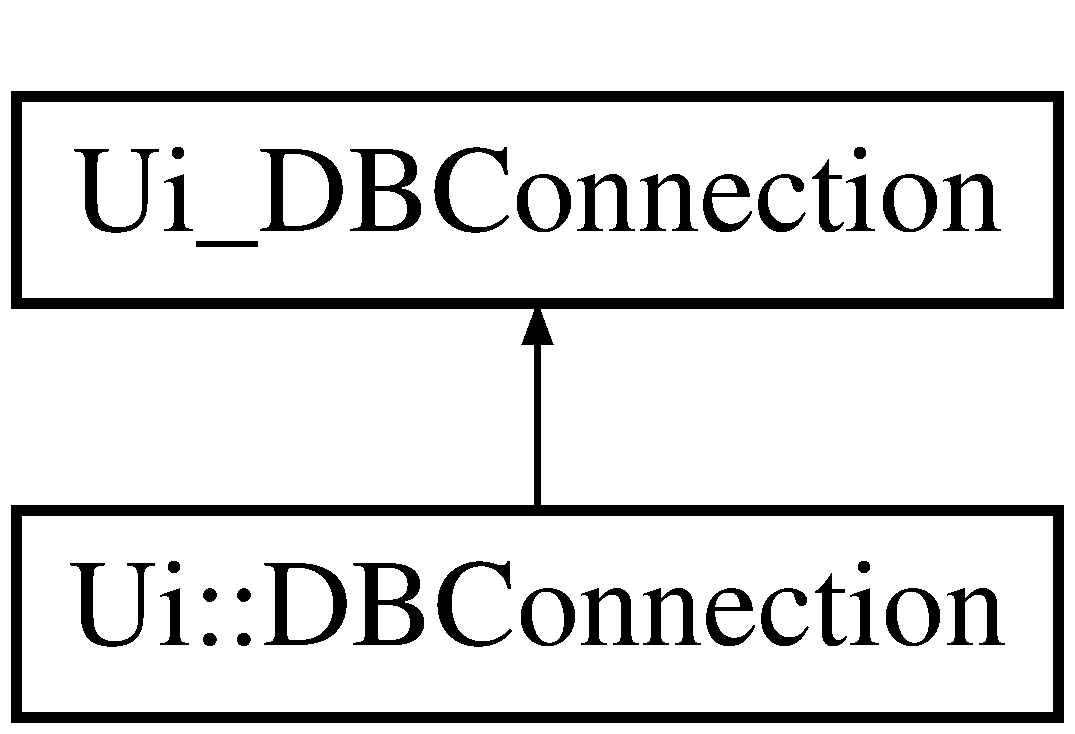
\includegraphics[height=2.000000cm]{classUi__DBConnection}
\end{center}
\end{figure}
\subsection*{Public Member Functions}
\begin{DoxyCompactItemize}
\item 
\hypertarget{classUi__DBConnection_acaf1a829dbcfeb5283bb65d04a190bf3}{void {\bfseries setup\-Ui} (Q\-Dialog $\ast$\hyperlink{classDBConnection}{D\-B\-Connection})}\label{classUi__DBConnection_acaf1a829dbcfeb5283bb65d04a190bf3}

\item 
\hypertarget{classUi__DBConnection_a7519839dbe5f8101d687a5ad6a58c600}{void {\bfseries retranslate\-Ui} (Q\-Dialog $\ast$\hyperlink{classDBConnection}{D\-B\-Connection})}\label{classUi__DBConnection_a7519839dbe5f8101d687a5ad6a58c600}

\end{DoxyCompactItemize}
\subsection*{Public Attributes}
\begin{DoxyCompactItemize}
\item 
\hypertarget{classUi__DBConnection_a58e4b7c10d7cc21090f4b1ce371ea1ff}{Q\-V\-Box\-Layout $\ast$ {\bfseries vertical\-Layout}}\label{classUi__DBConnection_a58e4b7c10d7cc21090f4b1ce371ea1ff}

\item 
\hypertarget{classUi__DBConnection_a3ec5814b07530b9e92fad39e0739b372}{Q\-Grid\-Layout $\ast$ {\bfseries grid\-Layout}}\label{classUi__DBConnection_a3ec5814b07530b9e92fad39e0739b372}

\item 
\hypertarget{classUi__DBConnection_ac250e54405208b9f68ac5de20d4a9b19}{Q\-Line\-Edit $\ast$ {\bfseries line\-Edit\-\_\-2}}\label{classUi__DBConnection_ac250e54405208b9f68ac5de20d4a9b19}

\item 
\hypertarget{classUi__DBConnection_a33b57e55566cc6f84252ba72113f17c9}{Q\-Label $\ast$ {\bfseries label\-\_\-3}}\label{classUi__DBConnection_a33b57e55566cc6f84252ba72113f17c9}

\item 
\hypertarget{classUi__DBConnection_a20d1bc3fbdad47f0288df9faf9137490}{Q\-Line\-Edit $\ast$ {\bfseries line\-Edit\-\_\-3}}\label{classUi__DBConnection_a20d1bc3fbdad47f0288df9faf9137490}

\item 
\hypertarget{classUi__DBConnection_ace4c31d3e66f7adc3755b173febdadeb}{Q\-Line\-Edit $\ast$ {\bfseries line\-Edit}}\label{classUi__DBConnection_ace4c31d3e66f7adc3755b173febdadeb}

\item 
\hypertarget{classUi__DBConnection_a927fa90924399ea08ef88163ba5fe673}{Q\-Label $\ast$ {\bfseries label\-\_\-2}}\label{classUi__DBConnection_a927fa90924399ea08ef88163ba5fe673}

\item 
\hypertarget{classUi__DBConnection_a45b71a2e523d34ad4862aafc96df3683}{Q\-Label $\ast$ {\bfseries label}}\label{classUi__DBConnection_a45b71a2e523d34ad4862aafc96df3683}

\item 
\hypertarget{classUi__DBConnection_a9a6172ea8a7b40554f069b968997b858}{Q\-Dialog\-Button\-Box $\ast$ {\bfseries button\-Box}}\label{classUi__DBConnection_a9a6172ea8a7b40554f069b968997b858}

\end{DoxyCompactItemize}


The documentation for this class was generated from the following file\-:\begin{DoxyCompactItemize}
\item 
ui\-\_\-dbconnection.\-h\end{DoxyCompactItemize}

\hypertarget{classUi__Dialog}{\section{Ui\-\_\-\-Dialog Class Reference}
\label{classUi__Dialog}\index{Ui\-\_\-\-Dialog@{Ui\-\_\-\-Dialog}}
}
Inheritance diagram for Ui\-\_\-\-Dialog\-:\begin{figure}[H]
\begin{center}
\leavevmode
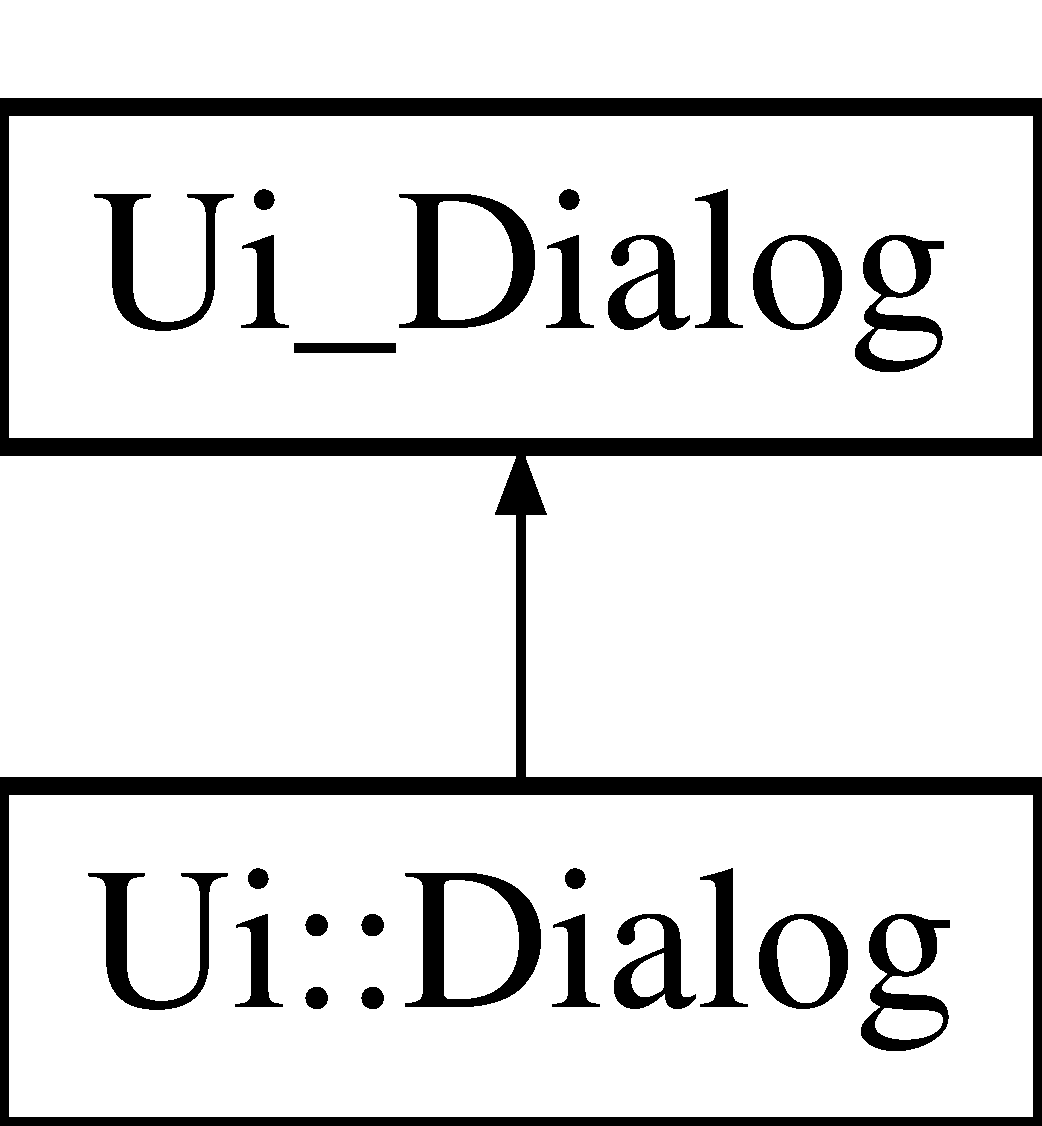
\includegraphics[height=2.000000cm]{classUi__Dialog}
\end{center}
\end{figure}
\subsection*{Public Member Functions}
\begin{DoxyCompactItemize}
\item 
\hypertarget{classUi__Dialog_a4f6a478c3ecdafabffb17b39cb26444a}{void {\bfseries setup\-Ui} (Q\-Dialog $\ast$Dialog)}\label{classUi__Dialog_a4f6a478c3ecdafabffb17b39cb26444a}

\item 
\hypertarget{classUi__Dialog_afa0ccb6f716ca6178260522a193c250e}{void {\bfseries retranslate\-Ui} (Q\-Dialog $\ast$Dialog)}\label{classUi__Dialog_afa0ccb6f716ca6178260522a193c250e}

\end{DoxyCompactItemize}
\subsection*{Public Attributes}
\begin{DoxyCompactItemize}
\item 
\hypertarget{classUi__Dialog_a02f973813b741621c5461918b3d9d4bb}{Q\-V\-Box\-Layout $\ast$ {\bfseries vertical\-Layout}}\label{classUi__Dialog_a02f973813b741621c5461918b3d9d4bb}

\item 
\hypertarget{classUi__Dialog_ae66a1da203f045e33d71ed5abd46d2a1}{Q\-H\-Box\-Layout $\ast$ {\bfseries horizontal\-Layout}}\label{classUi__Dialog_ae66a1da203f045e33d71ed5abd46d2a1}

\item 
\hypertarget{classUi__Dialog_a5f31f3804071e6b2008a98e72be07cc3}{Q\-Table\-View $\ast$ {\bfseries table\-View}}\label{classUi__Dialog_a5f31f3804071e6b2008a98e72be07cc3}

\item 
\hypertarget{classUi__Dialog_aebeace7895da27076f8f90c301742ec3}{Q\-Push\-Button $\ast$ {\bfseries push\-Button}}\label{classUi__Dialog_aebeace7895da27076f8f90c301742ec3}

\item 
\hypertarget{classUi__Dialog_a271a59402f80983c2722bb455db37365}{Q\-Dialog\-Button\-Box $\ast$ {\bfseries button\-Box}}\label{classUi__Dialog_a271a59402f80983c2722bb455db37365}

\end{DoxyCompactItemize}


The documentation for this class was generated from the following file\-:\begin{DoxyCompactItemize}
\item 
ui\-\_\-dialog.\-h\end{DoxyCompactItemize}

\hypertarget{classUi__NewDB}{\section{Ui\-\_\-\-New\-D\-B Class Reference}
\label{classUi__NewDB}\index{Ui\-\_\-\-New\-D\-B@{Ui\-\_\-\-New\-D\-B}}
}
Inheritance diagram for Ui\-\_\-\-New\-D\-B\-:\begin{figure}[H]
\begin{center}
\leavevmode
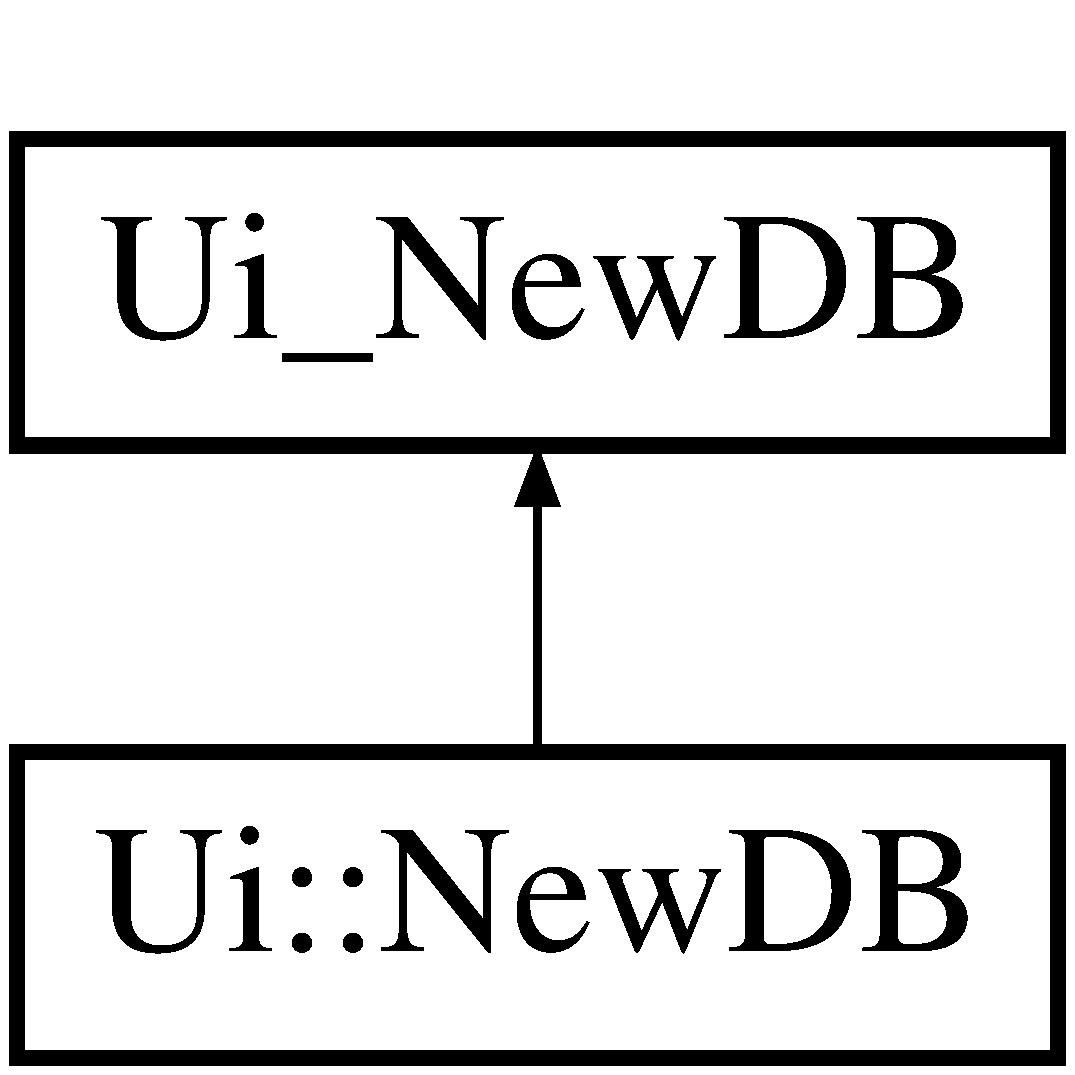
\includegraphics[height=2.000000cm]{classUi__NewDB}
\end{center}
\end{figure}
\subsection*{Public Member Functions}
\begin{DoxyCompactItemize}
\item 
\hypertarget{classUi__NewDB_a987269e012c9efceb2e7be46918b4823}{void {\bfseries setup\-Ui} (Q\-Dialog $\ast$\hyperlink{classNewDB}{New\-D\-B})}\label{classUi__NewDB_a987269e012c9efceb2e7be46918b4823}

\item 
\hypertarget{classUi__NewDB_a88d03cb02f4e00a0a517d33c8faf0b5c}{void {\bfseries retranslate\-Ui} (Q\-Dialog $\ast$\hyperlink{classNewDB}{New\-D\-B})}\label{classUi__NewDB_a88d03cb02f4e00a0a517d33c8faf0b5c}

\end{DoxyCompactItemize}
\subsection*{Public Attributes}
\begin{DoxyCompactItemize}
\item 
\hypertarget{classUi__NewDB_a9dff76495d9c01ca0adb6d4ae5647fbc}{Q\-V\-Box\-Layout $\ast$ {\bfseries vertical\-Layout}}\label{classUi__NewDB_a9dff76495d9c01ca0adb6d4ae5647fbc}

\item 
\hypertarget{classUi__NewDB_a754bb2ccd4cd7381d195e608e1a03e3d}{Q\-Grid\-Layout $\ast$ {\bfseries grid\-Layout}}\label{classUi__NewDB_a754bb2ccd4cd7381d195e608e1a03e3d}

\item 
\hypertarget{classUi__NewDB_ab5a707520470bc1b0506b2592991cf41}{Q\-Label $\ast$ {\bfseries label\-\_\-2}}\label{classUi__NewDB_ab5a707520470bc1b0506b2592991cf41}

\item 
\hypertarget{classUi__NewDB_a018bc89bfd201f79d0b6f83376b8d1dd}{Q\-Label $\ast$ {\bfseries label\-\_\-3}}\label{classUi__NewDB_a018bc89bfd201f79d0b6f83376b8d1dd}

\item 
\hypertarget{classUi__NewDB_a0b7cbad149393be2d42a55f35aa6a41d}{Q\-Label $\ast$ {\bfseries label}}\label{classUi__NewDB_a0b7cbad149393be2d42a55f35aa6a41d}

\item 
\hypertarget{classUi__NewDB_a22d07c33cac979fc1027a879682a77ca}{Q\-H\-Box\-Layout $\ast$ {\bfseries horizontal\-Layout}}\label{classUi__NewDB_a22d07c33cac979fc1027a879682a77ca}

\item 
\hypertarget{classUi__NewDB_a5b50844721eb57715bce1132baa71e38}{Q\-Line\-Edit $\ast$ {\bfseries line\-Edit\-\_\-2}}\label{classUi__NewDB_a5b50844721eb57715bce1132baa71e38}

\item 
\hypertarget{classUi__NewDB_a8a56adbfd095638426e4975443fee2db}{Q\-Line\-Edit $\ast$ {\bfseries line\-Edit\-\_\-3}}\label{classUi__NewDB_a8a56adbfd095638426e4975443fee2db}

\item 
\hypertarget{classUi__NewDB_a33e0b50acfaed1a733c62c2cd5f92b72}{Q\-Line\-Edit $\ast$ {\bfseries line\-Edit}}\label{classUi__NewDB_a33e0b50acfaed1a733c62c2cd5f92b72}

\item 
\hypertarget{classUi__NewDB_a40da91647c833ca87bbe290d7b615af4}{Q\-H\-Box\-Layout $\ast$ {\bfseries horizontal\-Layout\-\_\-2}}\label{classUi__NewDB_a40da91647c833ca87bbe290d7b615af4}

\item 
\hypertarget{classUi__NewDB_ae8390e64d2d1853f230cefa070a1ac0f}{Q\-Line\-Edit $\ast$ {\bfseries line\-Edit\-\_\-4}}\label{classUi__NewDB_ae8390e64d2d1853f230cefa070a1ac0f}

\item 
\hypertarget{classUi__NewDB_a82e635aa3dd0a99cec073c7ab3fa0200}{Q\-H\-Box\-Layout $\ast$ {\bfseries horizontal\-Layout\-\_\-3}}\label{classUi__NewDB_a82e635aa3dd0a99cec073c7ab3fa0200}

\item 
\hypertarget{classUi__NewDB_a8d4a8cc4028132a3621d085b162f356e}{Q\-Line\-Edit $\ast$ {\bfseries line\-Edit\-\_\-5}}\label{classUi__NewDB_a8d4a8cc4028132a3621d085b162f356e}

\item 
\hypertarget{classUi__NewDB_a26adf2500c8747bdf47f25f8318ce7a0}{Q\-Dialog\-Button\-Box $\ast$ {\bfseries button\-Box}}\label{classUi__NewDB_a26adf2500c8747bdf47f25f8318ce7a0}

\end{DoxyCompactItemize}


The documentation for this class was generated from the following file\-:\begin{DoxyCompactItemize}
\item 
ui\-\_\-newdb.\-h\end{DoxyCompactItemize}

\hypertarget{classUi__PlayerDialog}{\section{Ui\-\_\-\-Player\-Dialog Class Reference}
\label{classUi__PlayerDialog}\index{Ui\-\_\-\-Player\-Dialog@{Ui\-\_\-\-Player\-Dialog}}
}
Inheritance diagram for Ui\-\_\-\-Player\-Dialog\-:\begin{figure}[H]
\begin{center}
\leavevmode
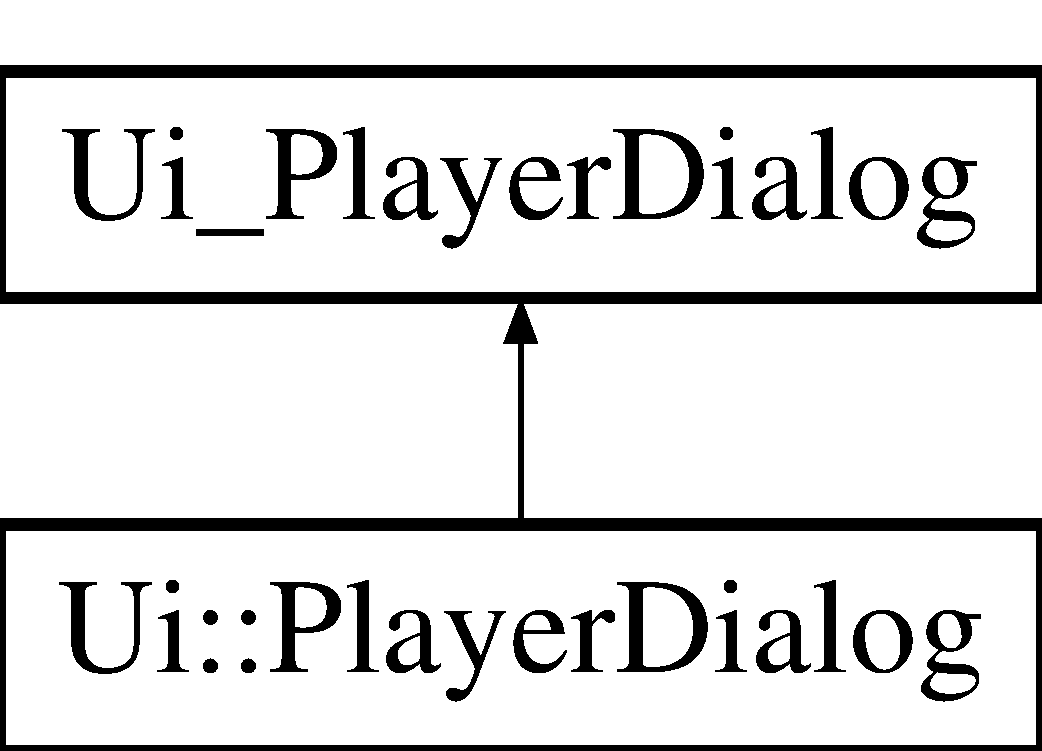
\includegraphics[height=2.000000cm]{classUi__PlayerDialog}
\end{center}
\end{figure}
\subsection*{Public Member Functions}
\begin{DoxyCompactItemize}
\item 
\hypertarget{classUi__PlayerDialog_a0ea34a28d6c510a07afc0abb0537767d}{void {\bfseries setup\-Ui} (Q\-Dialog $\ast$\hyperlink{classPlayerDialog}{Player\-Dialog})}\label{classUi__PlayerDialog_a0ea34a28d6c510a07afc0abb0537767d}

\item 
\hypertarget{classUi__PlayerDialog_aba529f69b1f8da81f43926c8116eb633}{void {\bfseries retranslate\-Ui} (Q\-Dialog $\ast$\hyperlink{classPlayerDialog}{Player\-Dialog})}\label{classUi__PlayerDialog_aba529f69b1f8da81f43926c8116eb633}

\end{DoxyCompactItemize}
\subsection*{Public Attributes}
\begin{DoxyCompactItemize}
\item 
\hypertarget{classUi__PlayerDialog_a74a12afbe6f09465dc1767c5868351f7}{Q\-V\-Box\-Layout $\ast$ {\bfseries vertical\-Layout\-\_\-2}}\label{classUi__PlayerDialog_a74a12afbe6f09465dc1767c5868351f7}

\item 
\hypertarget{classUi__PlayerDialog_afab06d2130637ccad71826f9888f1e08}{Q\-V\-Box\-Layout $\ast$ {\bfseries vertical\-Layout}}\label{classUi__PlayerDialog_afab06d2130637ccad71826f9888f1e08}

\item 
\hypertarget{classUi__PlayerDialog_a1cb63a2779b36cced50dfc985d20ed7b}{Q\-H\-Box\-Layout $\ast$ {\bfseries horizontal\-Layout}}\label{classUi__PlayerDialog_a1cb63a2779b36cced50dfc985d20ed7b}

\item 
\hypertarget{classUi__PlayerDialog_a656e4cebd17a01eee97530f41b1d6bf5}{Q\-Label $\ast$ {\bfseries label}}\label{classUi__PlayerDialog_a656e4cebd17a01eee97530f41b1d6bf5}

\item 
\hypertarget{classUi__PlayerDialog_a872ef92a5dd2eaeff2359e7adf03a4b6}{Q\-Line\-Edit $\ast$ {\bfseries line\-Edit}}\label{classUi__PlayerDialog_a872ef92a5dd2eaeff2359e7adf03a4b6}

\item 
\hypertarget{classUi__PlayerDialog_a0cc8a928a185491f8fe3a6cff4091f15}{Q\-H\-Box\-Layout $\ast$ {\bfseries horizontal\-Layout\-\_\-2}}\label{classUi__PlayerDialog_a0cc8a928a185491f8fe3a6cff4091f15}

\item 
\hypertarget{classUi__PlayerDialog_a78c550de67687e19505fc3c851e339f7}{Q\-Label $\ast$ {\bfseries label\-\_\-2}}\label{classUi__PlayerDialog_a78c550de67687e19505fc3c851e339f7}

\item 
\hypertarget{classUi__PlayerDialog_a3cd2d4e9c29c77c90b34ec0fdfcf8357}{Q\-Line\-Edit $\ast$ {\bfseries line\-Edit\-\_\-2}}\label{classUi__PlayerDialog_a3cd2d4e9c29c77c90b34ec0fdfcf8357}

\item 
\hypertarget{classUi__PlayerDialog_a3078a35028ed550f8a1f89e7af4d4663}{Q\-Spacer\-Item $\ast$ {\bfseries horizontal\-Spacer\-\_\-2}}\label{classUi__PlayerDialog_a3078a35028ed550f8a1f89e7af4d4663}

\item 
\hypertarget{classUi__PlayerDialog_abdb8e59012e0547e5ee4fcbd31c5d123}{Q\-Group\-Box $\ast$ {\bfseries group\-Box}}\label{classUi__PlayerDialog_abdb8e59012e0547e5ee4fcbd31c5d123}

\item 
\hypertarget{classUi__PlayerDialog_aab7e1fcb20ea71458e6eb77f177456f8}{Q\-H\-Box\-Layout $\ast$ {\bfseries horizontal\-Layout\-\_\-3}}\label{classUi__PlayerDialog_aab7e1fcb20ea71458e6eb77f177456f8}

\item 
\hypertarget{classUi__PlayerDialog_a1371a8148278463d57100b9eb8ddb659}{Q\-Radio\-Button $\ast$ {\bfseries radio\-Button}}\label{classUi__PlayerDialog_a1371a8148278463d57100b9eb8ddb659}

\item 
\hypertarget{classUi__PlayerDialog_a4b9bdb7af51ebed981c239e7f4e30298}{Q\-Radio\-Button $\ast$ {\bfseries radio\-Button\-\_\-2}}\label{classUi__PlayerDialog_a4b9bdb7af51ebed981c239e7f4e30298}

\item 
\hypertarget{classUi__PlayerDialog_a9d546737006452271099df6c12c26ea0}{Q\-Spacer\-Item $\ast$ {\bfseries horizontal\-Spacer}}\label{classUi__PlayerDialog_a9d546737006452271099df6c12c26ea0}

\item 
\hypertarget{classUi__PlayerDialog_ab775dc17461fb56eb9a722a1958ed4df}{Q\-Dialog\-Button\-Box $\ast$ {\bfseries button\-Box}}\label{classUi__PlayerDialog_ab775dc17461fb56eb9a722a1958ed4df}

\end{DoxyCompactItemize}


The documentation for this class was generated from the following file\-:\begin{DoxyCompactItemize}
\item 
ui\-\_\-playerdialog.\-h\end{DoxyCompactItemize}

\hypertarget{classUi__PlayersControl}{\section{Ui\-\_\-\-Players\-Control Class Reference}
\label{classUi__PlayersControl}\index{Ui\-\_\-\-Players\-Control@{Ui\-\_\-\-Players\-Control}}
}
Inheritance diagram for Ui\-\_\-\-Players\-Control\-:\begin{figure}[H]
\begin{center}
\leavevmode
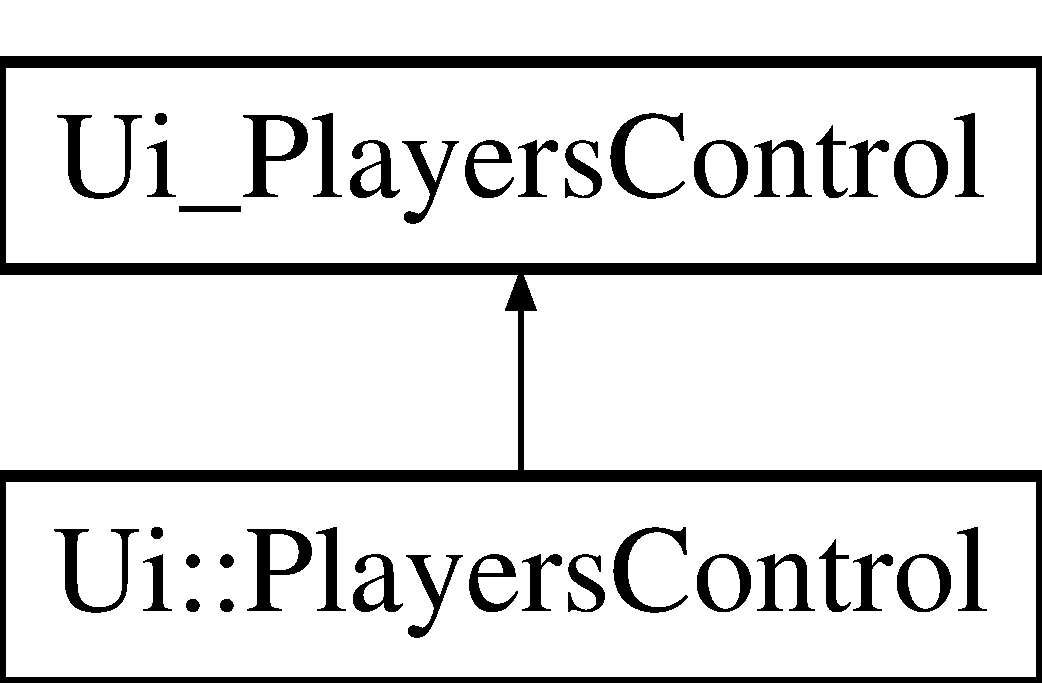
\includegraphics[height=2.000000cm]{classUi__PlayersControl}
\end{center}
\end{figure}
\subsection*{Public Member Functions}
\begin{DoxyCompactItemize}
\item 
\hypertarget{classUi__PlayersControl_a6acf9aeb42d67b31fc6e0bf5acf83539}{void {\bfseries setup\-Ui} (Q\-Dialog $\ast$\hyperlink{classPlayersControl}{Players\-Control})}\label{classUi__PlayersControl_a6acf9aeb42d67b31fc6e0bf5acf83539}

\item 
\hypertarget{classUi__PlayersControl_a8d9e5d1a31b87bfa71b6f5c8b0e0cbf9}{void {\bfseries retranslate\-Ui} (Q\-Dialog $\ast$\hyperlink{classPlayersControl}{Players\-Control})}\label{classUi__PlayersControl_a8d9e5d1a31b87bfa71b6f5c8b0e0cbf9}

\end{DoxyCompactItemize}
\subsection*{Public Attributes}
\begin{DoxyCompactItemize}
\item 
\hypertarget{classUi__PlayersControl_a6f41ca85309d3dc85fc7967086293793}{Q\-V\-Box\-Layout $\ast$ {\bfseries vertical\-Layout}}\label{classUi__PlayersControl_a6f41ca85309d3dc85fc7967086293793}

\item 
\hypertarget{classUi__PlayersControl_a44c0a411a5e03f2b3c01128501d574a3}{Q\-Tab\-Widget $\ast$ {\bfseries tab\-Widget}}\label{classUi__PlayersControl_a44c0a411a5e03f2b3c01128501d574a3}

\item 
\hypertarget{classUi__PlayersControl_a53966cce9febd1886aaf8589645cbcbc}{Q\-Widget $\ast$ {\bfseries tab\-\_\-2}}\label{classUi__PlayersControl_a53966cce9febd1886aaf8589645cbcbc}

\item 
\hypertarget{classUi__PlayersControl_afce8311ae458be25eb2cdd5e802fe6bc}{Q\-V\-Box\-Layout $\ast$ {\bfseries vertical\-Layout\-\_\-3}}\label{classUi__PlayersControl_afce8311ae458be25eb2cdd5e802fe6bc}

\item 
\hypertarget{classUi__PlayersControl_a9367d104230ed9257ee7c70fe9223225}{Q\-Table\-Widget $\ast$ {\bfseries table\-Widget\-\_\-2}}\label{classUi__PlayersControl_a9367d104230ed9257ee7c70fe9223225}

\item 
\hypertarget{classUi__PlayersControl_a5148bd66abd2161753c079e335ca9689}{Q\-H\-Box\-Layout $\ast$ {\bfseries horizontal\-Layout}}\label{classUi__PlayersControl_a5148bd66abd2161753c079e335ca9689}

\item 
\hypertarget{classUi__PlayersControl_a0f91fa1017b529a7a2937ff1edca4801}{Q\-Label $\ast$ {\bfseries label}}\label{classUi__PlayersControl_a0f91fa1017b529a7a2937ff1edca4801}

\item 
\hypertarget{classUi__PlayersControl_aaf3a7b641b749d84de2897b6da2df7ba}{Q\-Line\-Edit $\ast$ {\bfseries line\-Edit}}\label{classUi__PlayersControl_aaf3a7b641b749d84de2897b6da2df7ba}

\item 
\hypertarget{classUi__PlayersControl_ab7633929bb99833d1d5a5936f4aecfa7}{Q\-H\-Box\-Layout $\ast$ {\bfseries horizontal\-Layout\-\_\-3}}\label{classUi__PlayersControl_ab7633929bb99833d1d5a5936f4aecfa7}

\item 
\hypertarget{classUi__PlayersControl_a108770d25374326cb8f0b4187e24fb3b}{Q\-Radio\-Button $\ast$ {\bfseries radio\-Button\-\_\-2}}\label{classUi__PlayersControl_a108770d25374326cb8f0b4187e24fb3b}

\item 
\hypertarget{classUi__PlayersControl_ae08f650de3ada3aee4574c26b1e7ee38}{Q\-Radio\-Button $\ast$ {\bfseries radio\-Button}}\label{classUi__PlayersControl_ae08f650de3ada3aee4574c26b1e7ee38}

\item 
\hypertarget{classUi__PlayersControl_a55796711c4a4ffa8b15b16d8edda9bd4}{Q\-Label $\ast$ {\bfseries label\-\_\-2}}\label{classUi__PlayersControl_a55796711c4a4ffa8b15b16d8edda9bd4}

\item 
\hypertarget{classUi__PlayersControl_a5dde1725760ebd0941f5f0699e1daf36}{Q\-Line\-Edit $\ast$ {\bfseries line\-Edit\-\_\-2}}\label{classUi__PlayersControl_a5dde1725760ebd0941f5f0699e1daf36}

\item 
\hypertarget{classUi__PlayersControl_a36d1723722eae8f4cad725dd409ece22}{Q\-Push\-Button $\ast$ {\bfseries push\-Button}}\label{classUi__PlayersControl_a36d1723722eae8f4cad725dd409ece22}

\item 
\hypertarget{classUi__PlayersControl_a643c6d4bed8306b915c7248a885eb04f}{Q\-Dialog\-Button\-Box $\ast$ {\bfseries button\-Box}}\label{classUi__PlayersControl_a643c6d4bed8306b915c7248a885eb04f}

\end{DoxyCompactItemize}


The documentation for this class was generated from the following file\-:\begin{DoxyCompactItemize}
\item 
ui\-\_\-playerscontrol.\-h\end{DoxyCompactItemize}

\hypertarget{classUi__SceneDialog}{\section{Ui\-\_\-\-Scene\-Dialog Class Reference}
\label{classUi__SceneDialog}\index{Ui\-\_\-\-Scene\-Dialog@{Ui\-\_\-\-Scene\-Dialog}}
}
Inheritance diagram for Ui\-\_\-\-Scene\-Dialog\-:\begin{figure}[H]
\begin{center}
\leavevmode
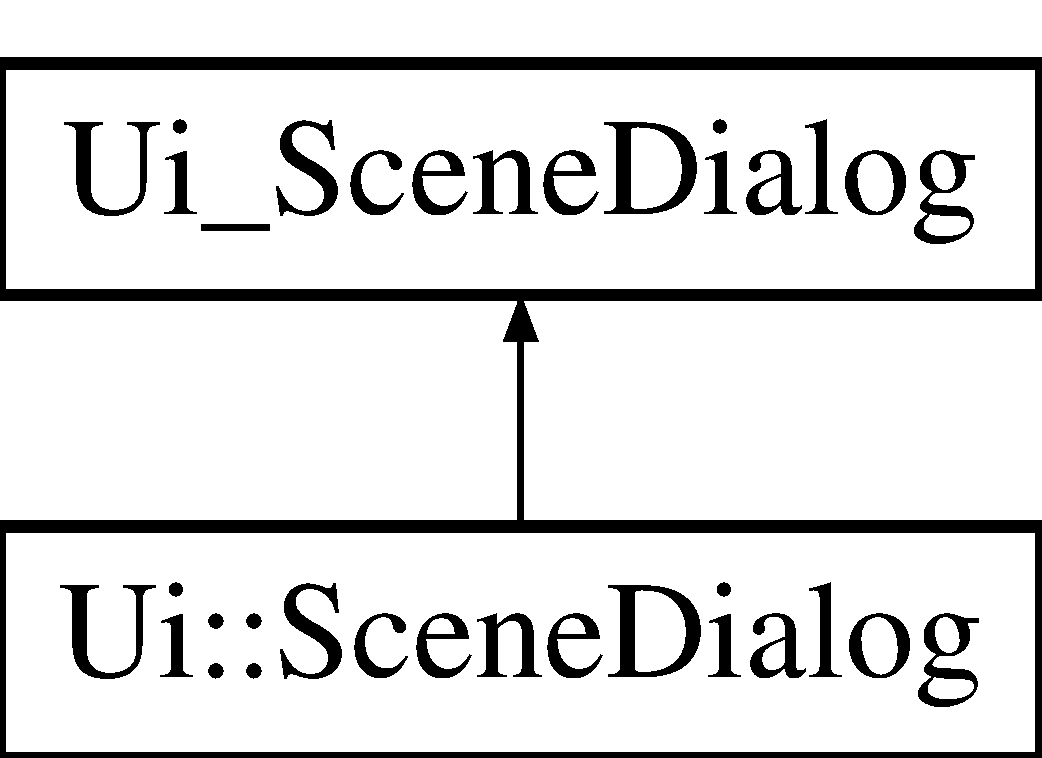
\includegraphics[height=2.000000cm]{classUi__SceneDialog}
\end{center}
\end{figure}
\subsection*{Public Member Functions}
\begin{DoxyCompactItemize}
\item 
\hypertarget{classUi__SceneDialog_a57bf95f881c27fd2fc2a8fdb9505f977}{void {\bfseries setup\-Ui} (Q\-Dialog $\ast$\hyperlink{classSceneDialog}{Scene\-Dialog})}\label{classUi__SceneDialog_a57bf95f881c27fd2fc2a8fdb9505f977}

\item 
\hypertarget{classUi__SceneDialog_a2e8cb0003e1d5f443bb3337d3237fabd}{void {\bfseries retranslate\-Ui} (Q\-Dialog $\ast$\hyperlink{classSceneDialog}{Scene\-Dialog})}\label{classUi__SceneDialog_a2e8cb0003e1d5f443bb3337d3237fabd}

\end{DoxyCompactItemize}
\subsection*{Public Attributes}
\begin{DoxyCompactItemize}
\item 
\hypertarget{classUi__SceneDialog_add94ac9bf68ea7783f29e7138a0d29ac}{Q\-V\-Box\-Layout $\ast$ {\bfseries vertical\-Layout}}\label{classUi__SceneDialog_add94ac9bf68ea7783f29e7138a0d29ac}

\item 
\hypertarget{classUi__SceneDialog_ac1c40b201004a216ff06a8ec7f85d441}{Q\-H\-Box\-Layout $\ast$ {\bfseries horizontal\-Layout}}\label{classUi__SceneDialog_ac1c40b201004a216ff06a8ec7f85d441}

\item 
\hypertarget{classUi__SceneDialog_a72db3f918483b57e410ec73936fba35f}{Q\-Label $\ast$ {\bfseries label}}\label{classUi__SceneDialog_a72db3f918483b57e410ec73936fba35f}

\item 
\hypertarget{classUi__SceneDialog_af510f91fc9536b2760f8414d4bc2ea8f}{Q\-Line\-Edit $\ast$ {\bfseries line\-Edit}}\label{classUi__SceneDialog_af510f91fc9536b2760f8414d4bc2ea8f}

\item 
\hypertarget{classUi__SceneDialog_a89117059c080378237d8de9029197438}{Q\-Dialog\-Button\-Box $\ast$ {\bfseries button\-Box}}\label{classUi__SceneDialog_a89117059c080378237d8de9029197438}

\end{DoxyCompactItemize}


The documentation for this class was generated from the following file\-:\begin{DoxyCompactItemize}
\item 
ui\-\_\-scenedialog.\-h\end{DoxyCompactItemize}

\printindex
\end{document}
